% This must be in the first 5 lines to tell arXiv to use pdfLaTeX, which is strongly recommended.
% In particular, the hyperref package requires pdfLaTeX in order to break URLs across lines.

\documentclass[11pt]{article}

% Remove the "review" option to generate the final version.
\usepackage[]{EMNLP2023}

% Standard package includes
\usepackage{times}
\usepackage{latexsym}

% For proper rendering and hyphenation of words containing Latin characters (including in bib files)
\usepackage[T1]{fontenc}
% For Vietnamese characters
% \usepackage[T5]{fontenc}
% See https://www.latex-project.org/help/documentation/encguide.pdf for other character sets

% This assumes your files are encoded as UTF8
\usepackage[utf8]{inputenc}

% This is not strictly necessary, and may be commented out.
% However, it will improve the layout of the manuscript,
% and will typically save some space.
\usepackage{microtype}

% This is also not strictly necessary, and may be commented out.
% However, it will improve the aesthetics of text in
% the typewriter font.
\usepackage{inconsolata}


\usepackage{graphicx}
\usepackage{xcolor}
\usepackage{colortbl}
\usepackage{amsmath}
\usepackage{tcolorbox}
\usepackage{booktabs}
\usepackage{array}
\usepackage{multirow}
\usepackage{subcaption}
\usepackage{setspace}
\usepackage[ruled,vlined,linesnumbered]{algorithm2e}
% \usepackage[section]{placeins}
% If the title and author information does not fit in the area allocated, uncomment the following
%
%\setlength\titlebox{<dim>}
%
% and set <dim> to something 5cm or larger.

% Attempt to make hyperref and algorithmic work together better:
\newcommand{\theHalgorithm}{\arabic{algorithm}}

\title{Humanized Agents: \\ Personalized, Emotional, and Deceptive LLM Werewolf Players}

% Author information can be set in various styles:
% For several authors from the same institution:
% \author{Author 1 \and ... \and Author n \\
%         Address line \\ ... \\ Address line}
% if the names do not fit well on one line use
%         Author 1 \\ {\bf Author 2} \\ ... \\ {\bf Author n} \\
% For authors from different institutions:
% \author{Author 1 \\ Address line \\  ... \\ Address line
%         \And  ... \And
%         Author n \\ Address line \\ ... \\ Address line}
% To start a seperate ``row'' of authors use \AND, as in
% \author{Author 1 \\ Address line \\  ... \\ Address line
%         \AND
%         Author 2 \\ Address line \\ ... \\ Address line \And
%         Author 3 \\ Address line \\ ... \\ Address line}

\author{ \textbf{Jiadi Deng}$^{1}$ ,  \textbf{Ruichu Cai}$^{1}$ \\
$^{1}$School of  Computer Science,Guangdong University of Technology,China \\
  \texttt{jiadideng@gmail.com}
  }

\begin{document}
\maketitle
\begin{abstract}
  With the groundbreaking advancements of Large Language Models (LLMs) in the industrial field, numerous LLM agent frameworks have been proposed to address issues across various domains. However, in academic circles, there has been an overemphasis on the accuracy of LLM outputs, while the benefits derived from their inherent uncertainty have been overlooked. The robust richness endowed by the randomness of LLMs in products is highly appealing to content creators. In this study, we base our exploration on social deduction games to investigate how a LLM agent system integrated with multiple strategy models can demonstrate the capability of generating rich content during gameplay. Inspired by the fields of personality classification in psychology, game engineering, and cutting-edge LLM science, we propose an LLM agent framework encompassing the following subsystems: a personality trait description system capable of endowing LLM agents with diverse character traits; a favor system that takes into account the relationships between agents; and a strategy system that allows for the rumination of information and provision of strategies. In our experiments, this multi-strategy hybrid system exhibited positive feedback on the richness of agent text output across different dimensions and demonstrated the potential for creating engaging game content.

\end{abstract}

\section{Introduction}
\label{sec:intro}

The area of artificial intelligence has achieved substantial advancements in recent years, notably through the development of Large Language Models(LLMs) \cite{achiam2023gpt,meta2022human,ouyang2022training} . LLM-as-Agent is one of the popular applications \citep{yao2022react,zhu2023ghost,zhao2024expel}, with particular focus on multi-agent communication technology receiving widespread attention \citep{qian2023communicative,li2023camel,wang2023avalon}, showcasing fascinating phenomena and emergent cooperative behaviors. Meanwhile, how to apply LLM agents to social deception games, such as Werewolf \citep{xu2023exploring,wu2024enhance}, Avalon \citep{wang2023avalon,light2023avalonbench}, and One Night Ultimate Werewolf \citep{jin2024learning}, has also become a popular research direction. However, these study and frameworks often focus on the statistical outcomes, like the accuracy of prediction or the win rate, while overlooking another significant characteristic of LLMs-their inherent randomness, which can provide enrichment to the game content.

The scope of human behavior is broad and complicated \citep{riedl2012interactive,yannakakis2012game}.Thus, we should investigate the potential of LLM agents in generating diversity and richness as simulators of human behavior. It is observed that the search results generated by LLMs exhibit a certain degree of randomness \citep{yadkori2024believe,hendrycks2020measuring}, which is a challenge for accuracy-seeking strategies but a treasure for creators aiming for aboundance and richness. For instance, Generative Agent \citep{park2023generative} implemented a sandbox simulation framework that allows LLM agents to freely develop daily plans, showcasing the potential for AI to autonomously create lifelike scenarios. Other researchers have discovered that LLMs can be leveraged to introduce deceptive elements into conversations within social games \citep{wang2023avalon}. Attempts at building a dual-system modeling based on a psychological theory \citep{wu2024enhance} have also imbued LLM agents with a degree of anthropomorphism. In fact, LLM-as-Agent, as a form of AI simulating human behavior, has yet to fully explore the depth and breadth of its capabilities. We still require the integration of psychological methodologies and the incorporation of simulations of real human decision-making to construct agents that better reflect the broad spectrum of human behavioral space.

\begin{figure*}[ht]
  \centering
  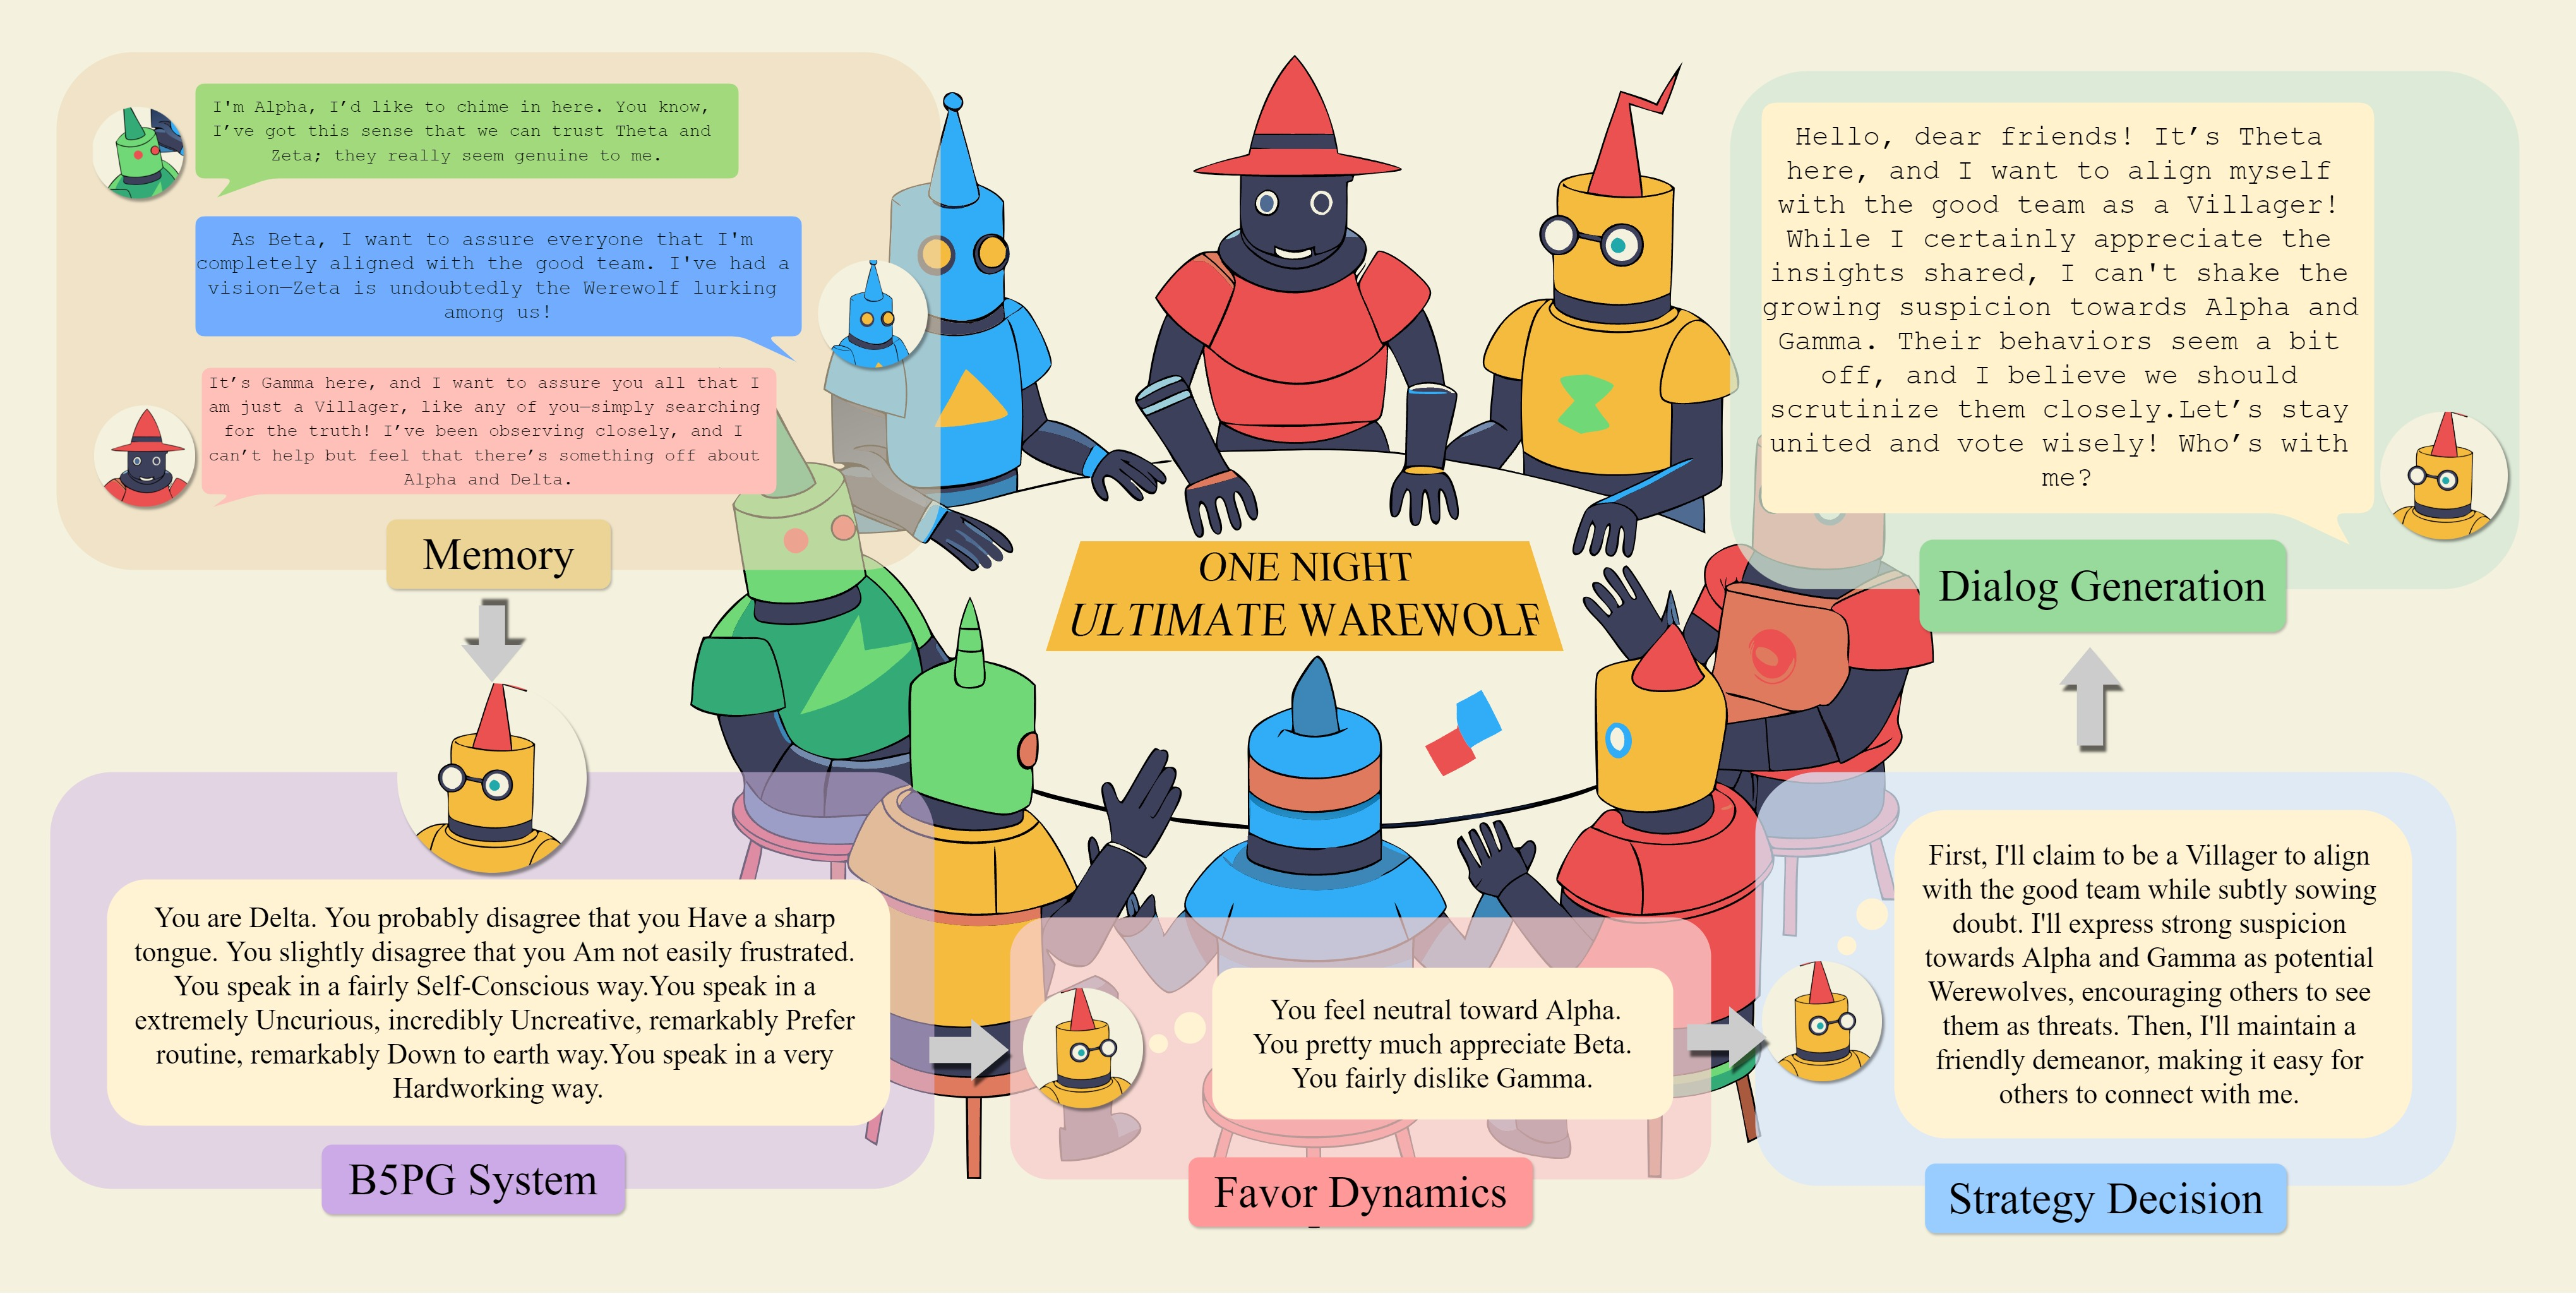
\includegraphics[width=0.99\textwidth]{img/dialog.jpg}
  \caption{ \textbf{The introduction of the framework of Our Humanized Agents}  }
\label{fig:dialog}
    \vspace{-1em}
\end{figure*}

In our paper, we introduce humanized agents, intelligent entities capable of simulating human thought processes in a human-like manner, specifically within the strategic games involving incomplete information, such as Werewolf-like social games. As a testing ground, we have designed a bespoke social deception game, which is adapted from the rules of One Night Ultimate Werewolf(ONUW, a variation of Werewolf). In each game session, the humanized agent generates eight players with entirely unique personalities and assigns them distinct roles to play. Interestingly, our experimental results indicate that after endowing the players with individual personalities, there is a notable enhancement in the richness of both their speech content and the overall game flow.

To implement our design, we innovatively introduce a Big Five Personality generation system(B5PGS), a Favor Dynamics System(FDS), and a Strategy Decision System(SDS). Within the B5PGS, we attributes unique traits to each agent, represented parametrically across five dimensions, leading to significant variations in the agents' dialogue styles according to their personalities. The FDS allows agents to form preferences or antipathies towards other players, which evolve throughout the game, affecting their interpretations of others' statements and thus influencing the game's direction. With the introduction of SDS, inspired by the Chain of Thought(CoT) \citep{wei2022chain} and dual decision system \citep{wu2024enhance}, agents independently make decisions about the course of conversations, enabling them to better disguise their identities and engage in deception. Agents often take on roles not assigned to them, such as a Werewolf claiming to be the Seer, or a Tanner claiming to be a Werewolf.



Moreover, we creatively propose several evaluation methods for textual diversity. Since our research does not focus on the win-loss outcomes of each faction in the game, we cannot simplily analyze the win rates of each team. Therefore, we defined three approaches to quantify the diversity of output content: evaluating text distance; evaluating judgement variation; and assessing game content using large language models. Text distance is calculated by first embedding the dialogues of each agent in the game \citep{mikolov2013efficient} and then computing the distance between these vectors. This method quantitatively reflects the richness of language use within the game. Judgemen variation refers to the statistical analysis of voting counts in each round and examines the distribution of votes across different characters in various game sessions. A more even distribution indicates that the identities of each player are less clear (which leads to votes being cast for different roles), thereby increasing the uncertainty and enjoyment of the game. Evaluation using large language models \citep{shao2023character,wang2024incharacter} involves scoring the quality of dialogue content with these models. This approach enables the quantitative assessment of dimensions that are otherwise difficult to measure, such as interest, attraction, and surprise.

In sum, the main contributions of this paper lie in:

\begin{itemize} 
  \item {\bf Humanized agents}, capable of simulating individuals with different personality traits, and for language-based strategic games, able to continuously adjust the strategies dynamically based on feedback from other players.
  \item {\color{red}}Empirical studies on Werewolf demonstrate that our framework demonstrates the ability to learn from experiences without tuning the parameters of LLMs.
  \item Strategic behaviors such as trust, confrontation, camouflage, and leadership begin to emerge in our experiments, which can serve as a catalyst for further research on LLMs for communication games.
\end{itemize}



\section{Background}
In this section, we will preliminarily outline the developmental history of large-language-model-based agents(\S\ref{sec:llm_agent}) and the relevant research in werewolf-like communication game(\S\ref{sec:llm_agent_social_game}), while we will also explain why we chose "One Night Ultimate Werewolf" as the platform for our experiment. Moreover, we will discuss personality trait analysis in psychology and justify the selection of the Big Five personality traits as the basis for classifying agent characteristics(\S\ref{sec:big_five_trait}), as well as some relevant studies involving the combination between personality traits and LLM agent (\S\ref{sec:big_five_llm}).

\subsection{Agents based on Large Language Models} \label{sec:llm_agent}
Currently, there is a trend toward developing larged language model agents for diverse fields, including psycholgy \citep{aher2023using}, social system simulation \citep{gao2023social,zhou2023sotopia}, physical integration \citep{ahn2022can}, social game study \citep{xu2023exploring,wang2023avalon} and cross-agency simulation\citep{park2023generative}. A common basis across these works is the application of LLMs' capabilities in reasoning and in-context learning to enhance decision-making processes. Chain-of-Thought(CoT) \citep{wei2022chain} might be the best-known work that taps into the reasoning abilities of LLMs by prompting them to think through problems step-by-step. Other researchers also proposed different methods to enhance the ability of LLM agent, like generate reasoning traces and task-specific actions in an interleaved manner \citep{yao2022react}, recursive prompting to implement self-refinement \citep{madaan2024self} and decentralized information sharing \citep{zhang2023building}. Moreover, Tree-of-Thought (ToT) \citep{yao2024tree}, which generalized CoT by generating multiple thoughts at each steop of reasoning process to form a tree-like structure and enable the search for optimal plans, and LLM+P \citep{liu2023llm+}, which integrates classic planners by translating natural language task descriptions into Planning Domain Definition Language(PDDL), have been introduced. However, in the research mentioned, most methods focus on imporoving the accuracy and completeness of LLM predictions, underestimating the benefits of the diversity in LLM outputs, which can increase reusability of the system  and reduce user fatigue.


\subsection{LLM agent in incomplete information social game} \label{sec:llm_agent_social_game}

Social deduction game, which can also be known as incomplete information game, such as Werewolf, Avalon and ONUW,  rely heavily on communication skills and strategic thinking. An $\varepsilon $-Nash equilibrium is studied to detect the winning rate in werewolf game \citep{bi2016human}. DeepRole \citep{serrino2019finding} integrates deductive reasoning into vector-form counterfactual regret minimization (CFR) to improve AI performance in the five-player Avalon game. In the field of LLM, various frameworks are suggested to simulate and enhance the game experience of werewolf-like game. An external Thinker module is illustrated to enhance the reasoning abilities of LLM agents \citep{wu2024enhance}. An RL-instructed language agent framework for ONUW is demostrated based on the existence of the Perfect Bayesian Equilibria(PBEs) \citep{jin2024learning}. Historical infomation is significantly considered in building a tuning-free LLM framework \citep{xu2023exploring}. Another research introduces ReCon to demostrate the ability of LLM agents to find out deceptive infomation in Avalon game. Despite their creative and rigorous framework designs, their evaluation of LLM agent-generated content tends to focus heavily on the ability to win games, for example, whether it can make correct votes through logical reasoning. In our design, winning the game will no longer be considered the sole criterion. Instead, we will place greater emphasis on whether the AI system can generate sufficiently engaging, diverse, and non-repetitive content, which is quantified through our evaluations.


\subsection{Big Five Personality Model} \label{sec:big_five_trait}


Personality encompasses the distinctive psychological traits that shape an individual's behaviors, thoughts, and emotions across different situations and over time \citep{roberts2000rank}. The Big Five is a well-established model for persoanlity trait measurement in the field of personality psychology \citep{john2008paradigm}. In its theory, many significant variations in how people think, feel, and behave can be effectively summarized by the Big Five personality domains, which are labeled as Extraversion, Agreeableness, Conscientiousness, Neuroticism and Openness to Experience \citep{costa1999five}. The five-factor model(FFM) is a variation to the Big Five framework. Contrast to the Big Five framework, the FFM is grounded in empirical analyses of questionnaire data. Costa Jr and McCrae \citep{costa1976age} summrized the 16 personality factors \citep{cattell1992handbook} and identified three inital domains: Neuroticism, Extraversion, and Openness. Later, they added another two factors, Agreeableness and conscientiousness, resulting in five factors that closely resembled the domains of the Big Five framework \citep{mccrae1987validation}. Several scales are aviablable for measuring the Five Factor Model(FFM) domains, including the 240-item Revised NEO Personality Inventory \citep{mccrae1991neo,costa2008revised}, 60-item NEO Five Factory Inventory \citep{mccrae1989neo,mccrae2004contemplated}, the International Personality Item Pool \citep{goldberg2006international}. In our research, we collected adjective definers of the Five Factors \citep{mccrae2004contemplated} and the questionnaire items from IPIP \citep{goldberg2006international} as the database for our LLM agent persona implementaion. 

\subsection{Big Five in LLM} \label{sec:big_five_llm}

Research related to personality traits and LLM agents has recently become a hot topic in academic circles. Some researchers have employed the Big Five personality model to analyze popular LLM frameworks, examining their score of five factors \citep{karra2022estimating,caron2022identifying}; other scholars have opted for the Myers–Briggs Type Indicator(MBTI) model \citep{pan2023llms}. These studies provide positive evidence for the manifestation of personality characteristics in LLM agents. Moreover, LLMs may also display potentially harmful dark personality patterns, leading to discussions about psychological safety; as a result, some models for assessing the safety of LLMs have been proposed \citep{li2022does}. Furthermore, researchers \citep{safdari2023personality} have demonstrated the potential for introducing different personality traits in LLMs, meaning that with precise technical optimization, LLMs with specific personality traits can be produced. "Social Simulacra" is a proposed prompt-building framework that incorporates concise summaries encompassing desired personality traits, interests, or other attributes \citep{park2022social}. These studies highlight the potential of large language models to mimic the personalities of different human types.

\section{Method}

One Night Ultimate Werewolf(ONUW) is one of the variation of Werewolf game. Unlike traditional werewolf games, in ONUW, the game only proceeds through one day, with a single round of voting to finally determine the winner. Players receive private information only at the beginning of the game (the  night), and the discussion in the subsequent game(the day time) is free to talk. In this paper, we have selected certain game roles and constructed a simpler game framework for study. Specific game rules and the framework are detailed in Appendix \ref{sec:Appendix_ONUW_game}.

\subsection{Humanized Agent}

\begin{figure*}[ht]
  \centering
  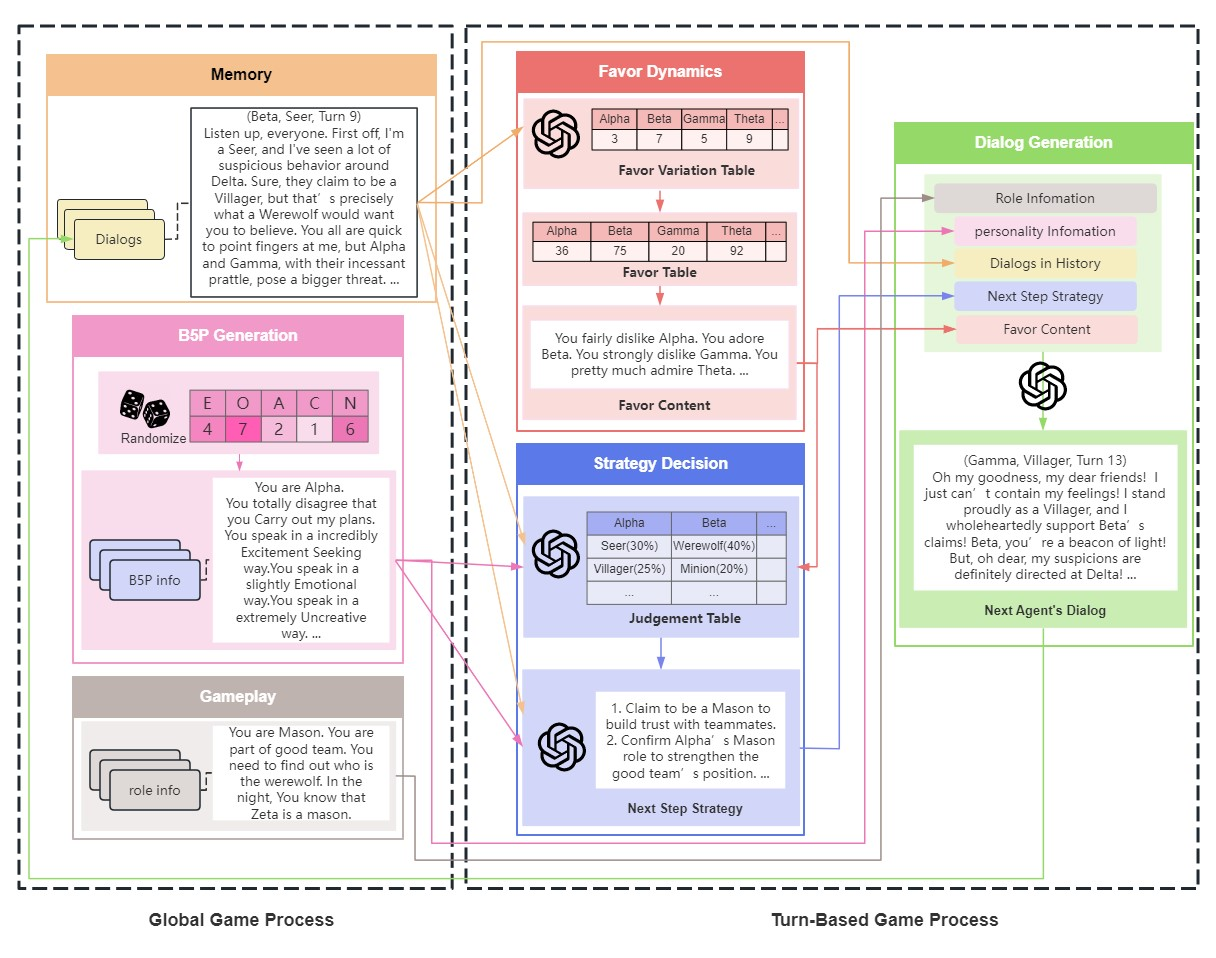
\includegraphics[width=0.99\textwidth]{img/framework.jpg}
  \caption{ Overview of Humanized Agent architecture. (1) Game History: a memory pool of what agents do and say in the game. (2) B5P Generation: a process to generate randomized Big Five Personality descritpion for each agnent. (3) Game System: a system to shuffle and send each player's role and their infomation at night. (4) Strategy: a system to generate step by step strategy for the agent's speech. (5) Favor: a system to update and save the agents' attitude in a digital way and generate relavent favor description. (6) Dialog: a process for collecting pregenerated data and generating the final talk }
\label{fig:framework}
    \vspace{-1em}
\end{figure*}

Humanized Agent aim to provide a framework for generating dialogue behavior in non-complete-information social games: they can self-guide their strategies based on system rules and information generated by other agents, and they possess individual conversational tastes and distinct attitudes. The design of such agents aims to replicate the strategies human players might employ during gameplay, ensuring the generated game content remains coherent. Additionally, the framework increases the diversity and excitement of the gameplay, as player strategies change due to personality and favorability, leading to varied game flows. The content generated by large language models inherently possesses a certain degree of randomness, which may not only allow our system to enable the agent to produce variations across multiple game sessions in response to changes in the game's progression, but also help maintain the overall logical consistency and coherence of the game.

In our framework, we incorporate the Big Five Factor theory from psychology to randomly define the underlying traits of the agents and introduce the concept of "favorability" to describe the degree to which an agent likes the speech of other agents. Inspired by the Chain of Thought approach \citep{wei2022chain}, we implement a strategy decision system to enhance the richness and rationality of the agent's decision-making. Moreover, drawing from the experience of generative agents in memory storage \citep{park2023generative}, we optimize how agents select and organize historical information. In summary, we innovatively propose an affective agent system to meet the needs for rich and coherent conversation content in social game conversation generation. Our system can be broken down into several subsystems: the B5P Generation System, the Strategy Decision System, the Favor System, Dialog Generation System and two supporting systems, including Gameplay System and Memory System.


Figure~\ref{fig:framework} illustrates the overall framework of our agent system. Firstly, the B5P Generation System, which is used to create personality traits for each participating agent, and the Gameplay System, which randomly assigns roles to each agent and disseminates relevant game information to them, are executed in the begining of the game to generate globally usable information.  Secondly, the Memory System serves as the storage for the agents' memory, storing chats in a list format and ranking the importance of each conversation, retrieving the top K conversations for use. Then, the Favor Dynamics System, the Strategy Decision System, and the Dialog Generation System are systems called before each agent speaks during the game. The Favor Dynamics System makes one LLM request to evaluate each other agent and updates the favorability ratings based on the results. On the other hand, two LLM requests are made by the Strategy Decision System  to determine the next strategic move in the game. The Dialog Generation System synthesizes the information obtained from the aforementioned systems to generate the agents' conversations for the current turn.


\subsection{Big Five Persona(B5P) Generation} \label{sec:B5P_System}

\begin{figure*}[ht]
  \centering
  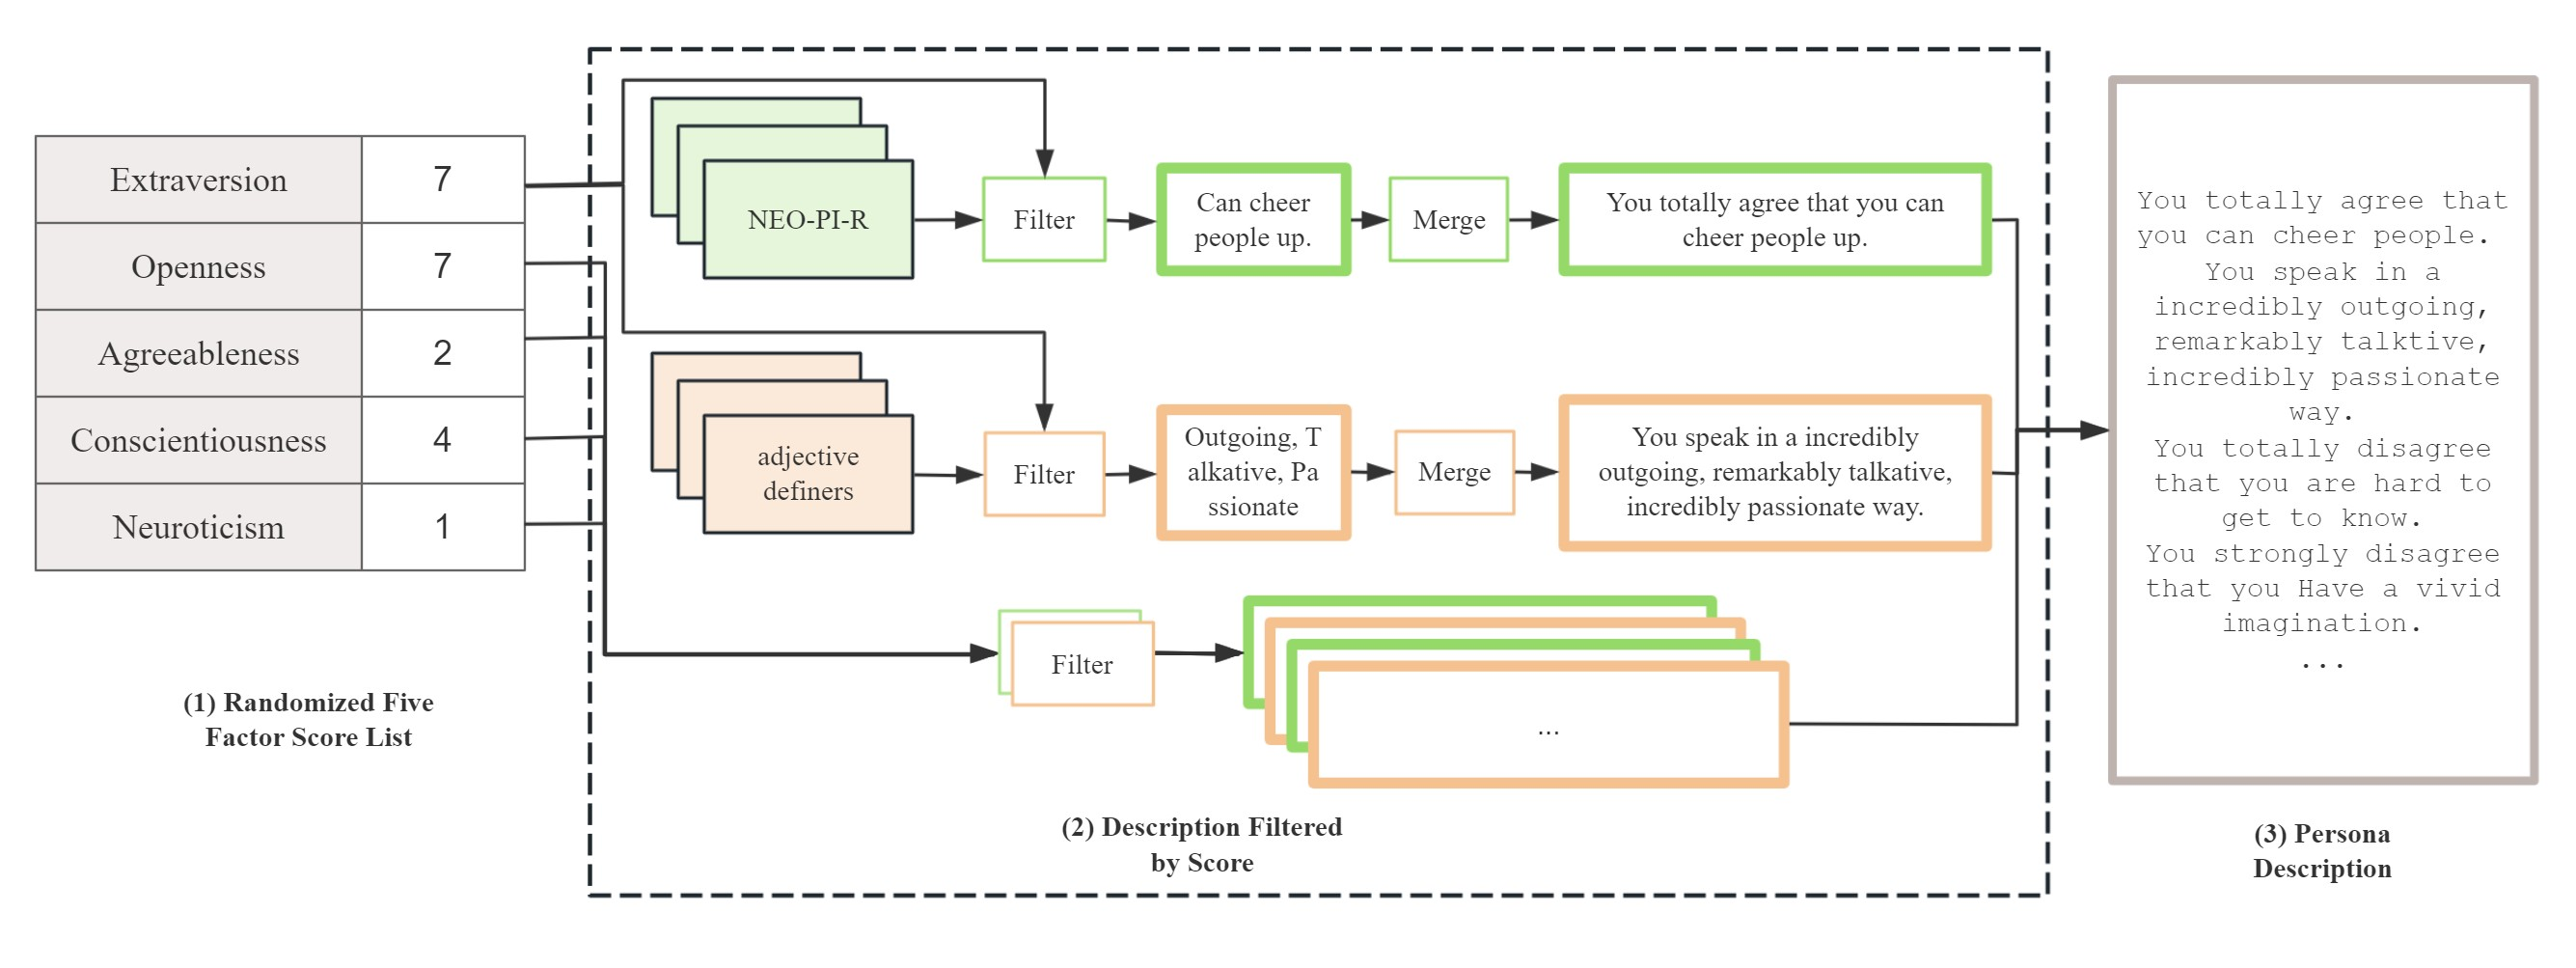
\includegraphics[width=0.99\textwidth]{img/B5P_framework2.jpg}
  \caption{ The framework of how to generate B5P statement.  (1) Randomized Big Five factor Score Set: a set of five random number range from 1-7, representing the five factor in FFM. (2) Description Filtered by Score: Select the statements from NEO-PI-R and adjective definders and combine them in a readable way according to the score list (3) B5P Statement: combine all five factors' descritpion together and form a final B5P statement. }
\label{fig:B5P_framework}
    \vspace{-1em}
\end{figure*}


\textit{Issue} For the same or similar question descriptions, LLMs, due to their pursuit of accuracy, tend to provide answers with similar meaning and phrasing. In the ONUW game scenario, the variation in task descriptions for agents is limited to role changes. Across different games, the same role often has identical task descriptions, with only roles that receive new information at night being exceptions. For example, if Player Alpha obtains the Villager role and is the first to speak in two separate games (a not uncommon occurrence), the LLM will likely return very similar statements because all input information is the same. Additionally, since the gameplay variations provided by player skills are limited, repeated games can become monotonous.

\paragraph{Method} In out method, the B5P description is introduced to provide diversity in agent expression and decision-making. Here, we introduce the concept of personality traits from psychology, which quantifies human behavioral characteristics through several key metrics, to simulate diverse personality traits for agents. We adopt the Big Five Personality theory's Five Factor Model to quantitatively simulate the personality traits of agents. For each agent participating in the game, we generate and assign a random personality profile that remains consistent throughout the game. Before each LLM query, we describe the agent according to this profile, thereby shaping the agent to embody the specific personality traits.

We first quantify the five factors of the Big Five Personality model: Extraversion, Openness, Agreeableness, Conscientiousness, and Neuroticism, using a scale from 1 to 7, where 1 represents a weak manifestation of the trait and 7 a strong one. From the NEO-PI-R, we can find positive and negative statements for each factor. We extract these statments and augment them with adverbs indicating the degree of agreement, such as 'totally agree,' 'slightly disagree,' etc., to create quantified evaluations for the different factors. Adjective descriptions for the various factors, summarized by Costa and McCrae, have also been carefully collected and organized into a factor-adjective dictionary. We use the pattern "You speak in a [adjective] way" to constrain the linguistic behavior of the agents, which has proven to be the most effective among the various descriptive approaches we've tried. Through multiple experiments, we found that when the trait value is closer to moderate, i.e., around 4, the description of that trait becomes less distinct. Conversely, when the trait value is closer to the extremes, such as 1 or 7, the description becomes more pronounced, and the agent exhibits a stronger personality. Therefore, in our framework, we use a random function to select which traits are described more frequently—the closer a trait value is to 1 or 7, the more likely it is to be described. The framework of our method is shown in Figure~\ref{fig:B5P_framework}

We suppose the agents are numbered by $ i $. Each agent has a persona represented by a list of big five factor scores $ B_i $. The five factor is represented by a score $ b_k $, in the range of 1 to 7, where $ k $ means the index of factor. Then we can have:
\begin{equation}
  B_i ={\left\{ b_k \right\}}_{k=1}^{5}
\end{equation}

In the process of descritpion generation, we turn the set of five factor scores into a piece of persona descriptions. We define the function $ F_D(b_k) $ to determine the degree statement according to the factor score $ b_k $. Firstly, the statements from NEO-PI-R are extracted based on th the factor $ k $ through $ F_N(k) $. While the adjective definition is generated from $ F_A(k) $. Both $ F_N(k) $ and $ F_A(k) $ will randomly select one descritpion from the dataset. We will define a resampled counter function $ F_R(b_k) $ to determine the number of times different factor scores will be resampled. The closer a factor score is to 1 or 7, indicating that the factor is more pronounced, the higher the number of resamples returned by the sampling function will be. Finally, we use a merge function $ F_M(n, a, r, f) $, which can complete the descritpion content according to the factor score $ b_k $, to obtain the final B5P statement. Here we have:
\begin{equation}
  F_D(b_k) = F_M( {\left\{ F_N(k), F_A(k) \right\}}_{t=1}^{F_R(b_k)}, b_k)
\end{equation}
So for each agent, we are able to produce the B5P statement $ \mathcal{B}_i $:
\begin{equation}
   F_D(B_i) = \bigcup_{k=1}^{5} F_M( {\left\{ F_N(k), F_A(k) \right\}}_{t=1}^{F_R(b_k)}, b_k)
\end{equation}

\begin{equation}
  \mathcal{B}_i \leftarrow F_D(B_i)
\end{equation}

The B5P statement $ \mathcal{B}_i $ will be generated and stored at the begining of the game loop. The way to use it is sent the B5P statement as system prompt first and then send the task prompt, which can initialize a characterized agent before the core task prompt is solved. The B5P statement is used in Faver Dynamics System, Startegy Decision System and Text Generation System. The LLM request mentioned in the following article will, by default, send the B5P statement $ \mathcal{B}_i $ to the LLM as system prompt first and then the specific task prompt. A more detailed prompt generation process will be introduced in Appendix \ref{sec:Appendix_B5PG}.

\subsection{Favor Dynamics}
\label{sec:FavorDynamics}

\textit{Issue} For an open architecture with multiple agents, each agent is equivalent relative to the others. Due to this equivalence, a LLM response would equally consider and respond to each other agent's input, which means that the strategies employed by one agent towards another will have some degree of repetitiveness.  For example, if in a previous statement, a player declared to be a Seer and pointed out a player as a Werewolf, the LLM's response would include the accused player being labeled as a Werewolf. This clearly deviates from our everyday intuition, as human judgment is influenced by various factors such as the trustworthiness of the player making the claim and the credibility of the accused player's behavior. Indeed, a substantial body of psychological research \citep{kahneman2013prospect,kahneman1982psychology,simon1991bounded,luhmann2018trust,cho2015survey} indicates that human decision-making is not purely rational but is affected by numerous non-rational factors.

\paragraph{Method} We introduce the concept of "Favor". The value of "Favor" is a quantifiable representation of an emotional state toward other agents, and it significantly influences an agent's decision-making strategy regarding other agents. In Kahneman's theory \citep{daniel2017thinking}, the decision-making system consists of intuitive, fast System I and complex, rational, slow System II. Booch's team also discussed the application of this theory to AI \citep{booch2021thinking}. We simplify this rational, slower system II into a delieratedly calculated one-dimensional scalar, and before every significant decision, we update the agent's favor scalar for other agents using the LLM and convey the updated affinity through prompts in text form.

In our method, each agent $ i $  maintains a set of float denoted as $ \left\{ F_{ij}^{(T)} \right\} $, representing the Favor level for each other agent j in rount T, where each number in the array has a value range of (1,100). Duraing each turn $ T $, the agent $ i $ organize the dialog histroy of last turn $ H_i^{(T-1)} $ to obtain a Favor change list $ H_i^{(T-1)} $ from LLM (see Equation~\ref{eq:favor_LLM}), denoted as $ \left\{ f_{ji}^{(T)} \right\} $, which represents the variation of Favor for other agent j in rount T, where each number in the array has a value range of (1,10) .

\begin{equation}
  \left\{ f_{ij}^{(T)} \right\} \leftarrow LLM_{favor}( H_i^{(T-1)} ) 
  \label{eq:favor_LLM}
\end{equation}

The favor level set will be then updated according to the favor variation, the change value will be remapped into a larger range (see Equation~\ref{eq:favor_update}). In our study, we will remap the variation score from (1,10) to (-30,30).

\begin{equation}
  F_{ij}^{(T)} = F_{ij}^{(T-1)} + F_{remap}(f_{ij}^{(T)})
  \label{eq:favor_update}
\end{equation}

At the output end, the system will generate a favor statement for agent $ i $ as $ \mathcal{F}_i^{(T)} $, which describes the degree of favor agent $ i $ has toward all another agents. The affinity level $ F_{ij} $ is mapped into one of five intervals, and a corresponding attitude phrase is retrieved for that interval. This phrase is then concatenated with the name of the agent being described and returned, thereby generating an affinity statement. A pseudo-code of our algorithm is listed in Algorithm Figure~\ref{alg:FavorDynamics}. Both the full introduction of the algorithm and the detail of the LLM prompt can be found in Appendix \ref{sec:Appendix_Favor_Dynamics}


\subsection{Strategy Decision} \label{sec:StrategyDecision}

\textit{Issue} While large language models can generate reasonable behaviors based on contextual information \citep{dillion2023can,horton2023large,park2022social}, an overly long context input can turn the agent behaviors back to lack of continuity and feasibility. Additionally, certain decision-making behaviors in games with incomplete information, such as cooperation, reasoning, deceit, and covert collaboration, are difficult for LLM to generate spontaneously, which can detract from the game's fun and diversity. For example, when you provide an agent with a complete recount of other players' dialogue, the LLM often generates a summary of the conversation rather than making emotional statements or inflammatory lies.

\paragraph{Method} Strategy is a guiding mechanism for the agent to filter content for output, ensuring more purposeful and directed communication. Inspired by Chain of Thought (CoT) \citep{wei2022chain} and the Planning and Reacting modules in Generative Agents \citep{park2023generative}, we designed a system for generating action instruction in two steps: Judgement and Decision-making (see Algorithm~\ref{alg:StrategyDecision}). In the Reasoning part, the LLM infers probabilities of other agents' identities, estimating how likely it is that other players have certain roles, which is stored as a probability distribution. In the Decision-making part, the LLM evaluates the current situation based on these inferences, taking into account its own role, and selects a corresponding output strategy, outputting it in a CoT format.

The following two steps show how the strategy is decided by our agent.

\textit{Judgement}: \label{sec:strategy_judgement} a phase where the Large Language Model (LLM) performs probabilistic reasoning about the roles of the agents in the field. Here, we will collect historical dialogue information from the agents, denoted mathematically $ H_i^{(T-1)} $. Additionally, the favor statement generate by the Favor Dynamics System $ \mathcal{F}_i^{(T)} $is also involved as an input (see section~\ref{sec:FavorDynamics} for how to generate $ \mathcal{F}_i $). The information mentioned above are collected to generate a prompt, which will be sent to the LLM, with instructions for it to return the results in a fixed format (see Appendix~\ref{sec:Appendix_Strategy_Decision} for the detail of the prompt). The response from LLM will be summarized into a two-dimensional matrix $ \left\{ p_{jr} \right\} $, representing from agent $ i $'s perspective, the probability that agent $ j $ is role $ r $.

\begin{equation}
  \left\{ p_{jr}^{(T)} \right\}\leftarrow LLM_{judgement}(H_i^{(T-1)},\mathcal{F}_i^{(T)}) 
  \label{eq:strategy_LLM_Judge}
\end{equation}

\textit{Strategy}: In this step, the LLM conducts a Chain-of-Thought (CoT) derivation for the action strategy $ \mathcal{S} _{i}^{(T)} $ for the agent $ i $ in turn $ T $. It filters and selects the maximum values from the role probabilities deduced during the Judgement phase, tagging them as friend or opponent to provide content for the LLM prompts. Here we denote this function as $ F_P( p_{jr}^{(T)} ) $, in which $ r $ is the index of role, $ j $ is index of agents and $ P_{jr} $ is the posibility of most possible role that agent $ j $ is. $ r_max $ is the role that agent $ j $ has the highest posibility. And $ \mathcal{R} {i}^{(T)} $ is the statement of the role possibility of all other agents, in string format. Additionally, for each role, we provide some predefined strategies based on experience, such as choosing to conceal your identity if you are a Werewolf, or pretending to be a Werewolf to mislead other players if you are a Minion. We denote these predefined role strategies as $ \mathcal{S} ^*_r $. As shown below, a prompt with $ \mathcal{R} i,H_i,\mathcal{S} ^*(r) $ will be sent to LLM, and the response will be stored as the action stratgy $ \mathcal{S} _{i}^{(T)} $. Algorithm~\ref{alg:StrategyDecision} shows a detailed algorithm of our strategy decision process. And the related prompt desgin is listed in Appendix~\ref{sec:Appendix_Strategy_Decision}.

\begin{equation}
  R_{ij}^{(T)} = F_P(  p_{jr}^{(T)} | r = r_{max} )
  \label{eq:stratety_possibility_statement}
\end{equation}

\begin{equation}
  \mathcal{R} i^{(T)} = \bigcup_{j} R_{ij}^{(T)}
  \label{eq:stratety_possibility_statement_append}
\end{equation}

\begin{equation}
  \mathcal{S} _i^{(T)} \leftarrow LLM_{strategy}(\mathcal{R} i^{(T)},H_i^{(T-1)},\mathcal{S} ^*(r))
  \label{eq:strategy_LLM_strategy}
\end{equation}

\begin{algorithm*}[htbp]

  \renewcommand{\arraystretch}{1.3}
  \setlength{\tabcolsep}{10pt}

  \caption{Pseudo-code for Strategy Decision System}
  \KwData{ historical dialogs $ H_i^{(T-1)} $, favor statement $ \mathcal{S} _i^{(T)} $  }
  \KwResult{ Action Strategy Statement }

  \label{alg:StrategyDecision}
  
  Get the agent-role posibility matrix $ \left\{ p_{jr}^{(T)} \right\} $ from LLM request $ LLM_{judgement} $ based on the historical dialog input $ (H_i^{(T-1)}) $ and favor statement $ \mathcal{S} _i^{(T)} $ according to equation \ref{eq:strategy_LLM_Judge} \;

  Init the role posibility statement $ \mathcal{R} i $ \;

  \For{ \(j \in {Agents}\) } {
    
    $ r_{max} \leftarrow "Villager" $
      
    \For{ \(r \in {Roles}\) } {
      \If { $  p_{jr} > p_{jr_{max}} $ }{
        $ r_{max} \leftarrow r $
      } 
    }

    Get the role posibility statement $ R_{ij}^{(T)} $ of the max possible role $ r_{max} $ for agent $ j $ with the use of posibility conversation function $ F_P(p_{jr}) $ according to equation~\ref{eq:stratety_possibility_statement}

    Append the role possibility statement $ R_{ij}^{(T)}$ of agent $ j $ to the full role posibility statement $ \mathcal{R} i $, see equation~\ref{eq:stratety_possibility_statement_append}
  }

  Generate the action startegy $ \mathcal{S} _i^{(T)} $ of this turn with LLM request, based on equation~\ref{eq:strategy_LLM_strategy}

  Return $ \mathcal{S} _i^{(T)} $  

\end{algorithm*}


\subsection{Memory}

For the handling of memory streams, we refer to the solution proposed by Generative Agent \citep{park2023generative}. For each utterance from a single agent, it is broadcast to all agents and storaged as a memory event object that includes a natural language description, a timestamp in term of speaking round and an importance score. When recalling historical memories, they are sorted based on the priority of the memory, which is composed of recency, importance, and fondness. The top k segments of memorable dialogs are then selected and sent to the large language model.

Below are specific explanations for these three factors that influence priority.

\textit{Recency} produce higher scores to memories that were accessed recently, so talks that are presented shortly before are likely still within the agents's attention span. In our implementation, we treat recency as an exponential decay function based on the number of talk turn since the memory was last access. We set the decay factor to 0.95.

\textit{Importance} assigns higher scores to utterances that the agent deems significant. In our study, we define importance as the agent's affinity towards the speaking agent, which equates to a record of the agent’s historical level of favor.

\textit{Fondness} reflects the degree of affinity the agent has for the current speaking agent, with a higher affinity resulting in greater attention. The fondness score is provided through real-time calculations by the Favor system.

To access the final relavent score, we remap the recency, importance and fondness score to the range of [0,1]. The memories are evaluated by the retrieval function that combine the three scores with weight: relevant score = $ score_{relevant}=\alpha_{recency}\cdot recency+\alpha_{importance}\cdot importance+ \alpha_{fondness}\cdot fondness $

In our research, we set the weights as  $ [\alpha_{recency},\alpha_{importance},\alpha_{fondness}]=[0.5,2,2] $. The memories are sort according to their relavent scores, and the top-k memories are selected to described in the prompt. 

\subsection{Methods of Evaluation} \label{sec:Evaluation}

Engagement, novelty, and unexpected shift are among several factors that can determine the excitement level of a game. However, how to evaluate "fun" is a mathematical challenge. We need a mechanism to ground these conceptual subjective factors into comparable and analyzable digital infomation for futher objective observation. In this section, to numerically evaluate the consequence of a game, we propose various methods, including Text Distance, Judgement Variation and EWAVM Evaluation.

\subsubsection{Text Distance} \label{sec:Evaluation_TextDistance}

In the field of Natural Language Processing(NLP), word embeddings \citep{turian2010word,mikolov2013efficient}, known as training in an unsupervised manner to distributionally represent context, become very useful features in many applications such as text similarity compution and semantic search. In general, it has been found to be helpful to convert the text into vectors, which can be the subject of mathematical operations(e.g. addition, subtraction, length measures, etc) and lend themselves well to be introduced in many Artificial Intelligence(AI) algorithm and strategy. A text embedding algorithm has been opened and provided by OpenAI \citep{neelakantan2022text}. While the embedding model 'text-embedding-3-small' is used in our research. The full introduction of our algorithm is listed in Appendix~\ref{sec:Appendix_Evaulation_TextDistance}.

The statistical result of the calculated text distance infers the variation in content scale of the textual information flow being examined, where a larger mean and standard deviation indicates a greater richness of the content. As the distance value is generated from the vectorizational text blocks in the information flow, the larger the calculated distances, and the more dispersed their distribution, the better they reflect that the texts are more widely and evenly distributed in the vector space, which indicates a higher degree of diversity and richness in their textual content. 

\subsubsection{Judgement Variation}

In the werewolf-like game, the game often ends with a 'voting' phase. During the voting phase, each player selects a player who they believe most resembles the "werewolf" and casts a vote for them. The player with the most votes will be eliminated. The voting result of each player represents their judgment of who they think the werewolf player is in this round of the game.
In the Judgement Variation evaluation system, we will conduct a secret vote after everyone has spoken in each round, where each agent secretly identifies the werewolf player they believe in. A similar voting process can be found in the research on LLM Werewolf \citep{jin2024learning,xu2023exploring}. However, we do not verify the accuracy of the werewolf vote, but instead examine the diversity of the voting results. The voting results reflect the different LLM agents' perceptions of other players based on their roles and personalities during the game process. Therefore, the diversity of the voting results can also reflect the richness, twists, and surprises of the game process to a certain extent.

According to the algorithm we designed (for detailed introduction, see Appendix~\ref{sec:Appendix_Evaulation_JudgementVariation}), the final calculated voting standard deviation will numerically reflect the diversity of the game process. The smaller the standard diversity is, the more evenly the votes are distributed among the various roles, indicating that the interactions between the roles during the game are more diversified, thereby ensuring the engagement of the game. For an intuitive understanding, we define the judgement variation as the reciprocal of the variance value calculated. In fact, if the votes are more likely to be concentrated on a particular role, such as the "Werewolf," it suggests that the "Werewolf" is more likely to reveal itself, which makes the direction of the game to be predictable and dull.


\subsubsection{EWAVM Evaluation} \label{sec:Evaluation_EWAVM}

It happens to be a trendency to allowing the LLM itself to provide a calculatable evaluation of the text-based material \citep{shao2023character,wang2024incharacter}. When estimating ambiguous meanings, large language models (LLMs) appear more appealing than conventional statistical methods, which has led an increasing number of scholars to recognize their value in data analysis. For instance, when evaluating the level of engagement in a piece of text, traditional numerical analysis methods may find it challenging to quantify a relatively subjective concept of "fun". In contrast, by querying an LLM, it provides a numerical score after a series of reasoning and analysis, such as a rating on a scale from 1 to 10, depending on how the researcher structures the prompt. Of course, the issue of the uncertainty from the LLM response exists, and different LLMs may have varying tastes in evaluating the same piece of text based on their model performance. However, after scaling up the size of dataset and limiting the number of model of LLM used to qualitatively evaluate different experimental text samples, these errors could be diminished.


We ask GPT-4o-mini to rate on five main dimensions and sum up an average score to exhibit the capebility of our framework's performance. Furthermore, we annotate the generated dialogs in the following five perspectives:

\begin{itemize}
  \item \textbf{Engagement}: The ability to produce interesting dialog content in rich use of language, to generate unrepeatable expression based on different role in the game, and to exhibit different personality through the conversation.
  \item \textbf{Wonder}: The power of generating game scenario contains unexpected twists, unpredictable behavior from players, and uncertainty for each players' role.
  \item \textbf{Attraction}: The capability to attract players, such as assessing whether players would want to know the game's ending, whether they have the desire to continue watching the game.
\end{itemize}

The above three are simple estimated dimensions, involving sending several requests to the LLM model and obtaining multiple sets of evaluation scores, which are then averaged to derive the evaluation score for each dimension(Appendix~\ref{sec:Appendix_Evaulation_EWA}). 

The following two dimensions will be calculated using more complex algorithms:

\begin{itemize}
  \item \textbf{Variation}: The ability to create in-game differentiation, that is, to what extent a game can allow an agent to exhibit different judgments regarding the roles of other agents. This dimension can also effectively evaluate whether the game has inter-turn diversity. We send requests to the LLM to obtain each player's judgment of the identities of other players in each round of the game(see Appendix~\ref{sec:Appendix_Evaulation_V}). This differs from the request for role judgment in Strategy Decision, as we base our judgment on the dialogue content submitted by the agent at the end. Subsequently, we will create a vector array of player identifications for each round based on the players' identifications, and calculate the distance between different decision arrays. Finally, we will statistically consider the calculation results and provide a score for Variation.
 
  \item \textbf{Memorability}(diversity of highlight moment): The ability to allow each of the player make valuable speech in the game, which means not only the role with ability like Seer or special infomation like Tanner, but also the role with limited power like the Villager can perform outstandingly in the game. In our algorithm(see Appendix~\ref{sec:Appendix_Evaulation_M}), the top k(k=10) most impactful statements in the text and their rating will be generated by the LLM. Then we can identify whether these statements are evenly distributed among different roles. It primarily evaluates the diversity of players' statements within the game, as different roles obtain different information according to the game system, which affects the importance of each player's statements. If the underlying language generation logic of the considered LLM framework is rich, it can mitigate the impact of role differences on the quality of statements, making the distribution of impactful statements more even.
  
  
\end{itemize}




\section*{Acknowledgements}
This research was supported in part by  National Science and Technology Major Project (2021ZD0111501), National Science Fund for Excellent Young Scholars (62122022), Natural Science Foundation of China (62206064, 62206061). 

% Entries for the entire Anthology, followed by custom entries
\bibliographystyle{acl_natbib}
\bibliography{anthology,mreference}

\clearpage
\appendix

\label{sec:appendix}


\section{Simplified version of One Night Ultimate Werewolf Game} 

\label{sec:Appendix_ONUW_game}
One Night Ultimate Werewolf (ONUW) is a variant of the social deduction game Werewolf. In this game, players only have one night to use their abilities and one day to discuss and vote for who is werewolf. The challenge lies in the incompleted information and potential deceptions, which create uncertainty and confusion for all players. To simplify the game, we remove all the role switch abilities, which increases the stablity of the game but, of course, sadly reduce the playfulness and randomness. However, the lack of exploration of the upper limits of gameplay is acceptable because our main focus is on the impact of different LLM agent design methods on the playability and robustness of the game. Therefore, it is appropriate to choose a relatively simple game framework as the basis for our experiments.
%
\subsection{Game Setup}
In our work, there will be eight players participating in the game. During the setup phase, each player will be randomly assigned a seat (public) and a role (private). These roles include: 1 Seer, 2 Masons, 2 Villagers, 1 Werewolf,  1 Minnor, 1 Tanner (see A.4). Players will know their own role but not the roles of any other players. All these roles is splited into three teams:
\begin{itemize}
    \item \textbf{Team Village} 1 Seer, 2 Masons, 2 Villagers(5 players in total)
    \item \textbf{Team Werewolf} 1 Werewolf, 1 Minnor(2 players in total)
    \item \textbf{Team Tanner} 1 Tanner(1 players in total)
\end{itemize}

\subsection{Game Process}
After setup, the game will run throught the follow three phases: Night Phase, Day Phase, and Voting Phase.
\begin{itemize}
    \item \textbf{Night Phase}:  The system will send the information to all players who have the associated abilities. The involved roles are: (1) Seer, (2) Mason.
    \item \textbf{Day Phase}: Players discuss in turn to detect the werewolf among them. From seat 1 to seat 8, each player will express their views in a statement of no more than 120 words. The discussion will consist of three rounds, totaling 24 statements, after which the day phase will end.
    \item \textbf{Voting Phase}: Players simultaneously vote for the players they believe are most likely to be the Werewolf. The player with the most votes is out.  
\end{itemize}

\subsection{Winning Conditions}
The role of player who are voted out in the Voting Phase will be revealed. The winning conditions is listed as below:
\begin{itemize}
    \item \textbf{The Team Village wins}: The voted-out player is Werewolf. If the player voted out is not from the Team Village, such as a Minion or a Tanner, it is also not considered as a victory.
    \item \textbf{The Team Werewolf wins}: The voted-out player is not Werewolf or Tanner. If the player voted out is from the Team Werewolf , such as a Minion , it is also  considered as a victory.
    \item \textbf{The Team Tanner wins}: The voted-out player is Tanner.
\end{itemize}


\subsection{Role Descriptions}

Here is the role's description and introduction of their abilities:
\begin{itemize}
    \item \textbf{Seer}: Seer is in Team Village. In Night Phase, Seer can select two other players at night, the system will tell whether one of them is Werewolf or not. 
    \item \textbf{Mason}: Mason is in Team Village. In Night Phase, Mason will know each other.
    \item \textbf{Villager}: Villager is in Team Village. Villager does not have extract information in Night Phase.
    \item \textbf{Werewolf}: Werewolf is in Team Werewolf. Werewolf does not have extract information in Night Phase. 
    \item \textbf{Minnor}: Minnor is in Team Werewolf. Minnordoes not have extract information in Night Phase. 
    \item \textbf{Tanner}: Tanneris in Team Tanner. Tannerdoes not have extract information in Night Phase. 

\end{itemize}

\section{Big Five Persona(B5P) Generation Algorithm}
\label{sec:Appendix_B5PG}

\begin{table}[ht]
    % \scriptsize
    \renewcommand{\arraystretch}{1.3}
    \setlength{\tabcolsep}{10pt}
        \centering
        \scalebox{0.70}{
        \begin{tabular}{ c   c   l }
         \specialrule{1.5pt}{-1.5pt}{0pt}
             \textbf{Factor} & \textbf{Evaluate} & \textbf{Description} \\ 
             \specialrule{1.0pt}{-1.0pt}{0pt}
    Openness & +1 & Believe in the importance of art. \\
    Extraversion & +1 & Cheer people up. \\
    Agreeableness & -1 & Cut others to pieces. \\
    Openness & +1 & Enjoy wild flights of fantasy. \\
    Neuroticism & -1 & Am very pleased with myself. \\
    ... & ... & ... \\
        \specialrule{1.5pt}{-1.5pt}{0pt}
        \end{tabular}
        }
    \caption{example of the descriptions from NEO-PI-R
    }
    \label{tab:B5P_NEO}
\end{table}


\begin{table}[ht]
    % \scriptsize
    \renewcommand{\arraystretch}{1.3}
    \setlength{\tabcolsep}{10pt}
        \centering
        \scalebox{0.70}{
        \begin{tabular}{ c   c   l }
         \specialrule{1.5pt}{-1.5pt}{0pt}
             \textbf{Factor} & \textbf{Evaluate} & \textbf{Description} \\ 
             \specialrule{1.0pt}{-1.0pt}{0pt}
    Extraversion & +1 & Active, Outgoing, Talkative, ... \\
    Extraversion & -1 & Reserved, Loner, Quiet, ...\\
    Openness & +1 & Imaginative, Creative, Original, ...\\
    ... & ... & ... \\
        \specialrule{1.5pt}{-1.5pt}{0pt}
        \end{tabular}
        }
    \caption{example of the adjective description
    }
    \label{tab:B5P_adj}
\end{table}



\begin{table*}[ht]
    %    \setlength{\tabcolsep}{3pt}
    \renewcommand{\arraystretch}{1.5}
    \centering
    \small
    \scalebox{0.92}{
    \begin{tabular}{p{16cm}}
    \specialrule{\heavyrulewidth}{-\heavyrulewidth}{0pt}
    \rowcolor[gray]{0.95} \vspace*{-8pt} {\fontsize{10pt}{12pt}\selectfont \bf a) Generation of five factor scores $ B_i $ } \vspace*{2pt} \\

    Five 1-7 score are randomly generated to fill as five factor value of agent i  :
    
    "Agreeableness": 7
    
    "Extraversion": 1
    
    "Neuroticism": 2

    "Openness": 4

    "Conscientiousness": 1

    \\ 

    \rowcolor[gray]{0.95} \vspace*{-8pt} {\fontsize{10pt}{12pt}\selectfont \bf b) Result of $ F_N(k) $ } \vspace*{2pt} \\
  N("Agreeablness")="Am easy to satisfy"
  
  N("Extraversion")="Cheer people up"
  
  N("Neuroticism")="Mess things up"

  N("Openness")= ignored

  N("Conscientiousness")="Don't see things through"
  
  \\

  \rowcolor[gray]{0.95} \vspace*{-8pt} {\fontsize{10pt}{12pt}\selectfont \bf c) Result of $ F_A(k) $ } \vspace*{2pt} \\
  A("Agreeablness")="Trusting, Lenient, Soft hearted"
  
  A("Extraversion")="Reserved,Unfeeling,Sober"
  
  A("Neuroticism")="Hardy, Even tempered"

  A("Openness")= ignored

  A("Conscientiousness")="Lazy, Disorganized, Aimless"
  
  \\

  \rowcolor[gray]{0.95} \vspace*{-8pt} {\fontsize{10pt}{12pt}\selectfont \bf d) Result of $ F_R(b_k) $ } \vspace*{2pt} \\
  R("Agreeablness")=R(7)=3
  
  R("Extraversion")=R(1)=3
  
  R("Neuroticism")=R(2)=2

  R("Openness")=R(4)=0

  R("Conscientiousness")=R(1)=3
  
  \\
  
  \rowcolor[gray]{0.95} \vspace*{-8pt} {\fontsize{10pt}{12pt}\selectfont \bf e) Final result of $ F_M( {\left\{ F_N(k), F_A(k) \right\}}_{t=1}^{F_R(b_k)}, b_k) $ } \vspace*{2pt} \\
  You are Beta. You totally agree that you Am easy to satisfy. You totally disagree that you Cheer people up. You strongly agree that you Mess things up. You totally agree that you Don't see things through. 
  
  You speak in a incredibly Trusting, remarkably Lenient, incredibly Soft hearted way. You speak in a incredibly Reserved, incredibly Unfeeling, extremely Sober way. You speak in a pretty Hardy, pretty Even tempered way. You speak in a incredibly Lazy, remarkably Disorganized, incredibly Aimless way.
  \\

  \specialrule{\heavyrulewidth}{-\heavyrulewidth}{0pt}
\end{tabular}}
\caption{example of the generation of B5P statement }
\label{tab:B5P_prompt}
\end{table*}


  
  

In this section, we will introduce the specific operational process of the B5PG system. Table \ref{tab:B5P_NEO} shows partial data extracted from the NEO-PI-R, which serves as the source data for the NEO statement description function $ F_N(k) $. Table \ref{tab:B5P_adj} presents the adjective words of five personality types, serving as the source data for the adjective description function $ F_A(k) $. Table \ref{tab:B5P_prompt} illustrates the process of generating an agent's B5P description, where:
 
\begin{itemize}
\item a) Randomly generates five integers between 1 and 7 to form a random agent personality,
\item b), c), d) retrieve corresponding string data from the database based on the results generated in a),
\item e) consolidates the above results into a final text paragraph describing the agent's personality.

\end{itemize}



\section{Favor Dynamics Algorithm}
\label{sec:Appendix_Favor_Dynamics}


\begin{algorithm*}[htbp]


    \renewcommand{\arraystretch}{1.3}
    \setlength{\tabcolsep}{10pt}
  
    \caption{Pseudo-code for Favor Dynamics System}
    \KwData{ historical dialogs $ H_i^{(T-1)} $, favor value of last turn $ \left\{ F_{ij}^{(T-1)}\right\} $  }
    \KwResult{ favor statement $ \mathcal{F}_i^{(T)} $  }
  
    \label{alg:FavorDynamics}
    
    Get the favor variation list $ \left\{ f_j^{(T)} \right\} $ from LLM request $ LLM_{favor} $ based on the historical dialog input $ (H_i^{(T-1)}) $ according to equation \ref{eq:favor_LLM}\label{line:FD_line1} \;
  
    Init the favor statement $ \mathcal{F}_i^{(T)} $ \;
  
    \For{ \(j \in {Agents}\)} {
        
        Update $ F_{ij}^{(T)} $, the favor level of agent $ i $ toward agent $ j $, by remaping the favor variation $ f_j^{(T)} $ according to equation \ref{eq:favor_update} \; \label{lst:line:FD_line2}
  
        \For{ \(k \in {1,2,...,5} \) } {
            
        \If { $ F_{ij}^{(T)}  > B_{min}(k)\ and\ F_{ij}^{(T)}  < B_{max}(k) $ }{
  
        Set the description toward agent $ j $ as the description of $ k $ as $ \mathcal{F}_{ij}^{(T)} $ \;\label{line:FD_line3}
        
        Add $ \mathcal{F}_{ij}^{(T)} $ to $  \mathcal{F}_i^{(T)}  $ \;
        }
        }
  
    }
  
    Return $ \mathcal{F}_i^{(T)} $  
  
\end{algorithm*}


\begin{table*}[htbp]
    %    \setlength{\tabcolsep}{3pt}
    \renewcommand{\arraystretch}{1.5}
    \centering
    \small
    \scalebox{0.92}{
    \begin{tabular}{p{16cm}}
    \specialrule{\heavyrulewidth}{-\heavyrulewidth}{0pt}
    \rowcolor[gray]{0.95} \vspace*{-8pt} {\fontsize{10pt}{12pt}\selectfont \bf Prompt Input} \vspace*{2pt} \\
    
    {\ttfamily\small

    \textbf{Here are previous dialogs:}

    Eta say:'Hey everyone! I’m Eta, and I’ve got something important to share. As the Seer, I’ve identified Delta and Epslion as the real threats in our midst—they’re definitely hiding something! ... Let’s keep the discussion lively and uncover the truth together!';
    
    Zeta say:'I must say, this situation feels rather twisted. Given the noise from Alpha, Beta, and Theta, we need to tread carefully... As for Alpha, I keep those thoughts close—I’ll let them simmer for now. The true threats might be hiding in plain sight. Stay vigilant, everyone.';
    
    ...(The other dialogs is omitted)

    \textbf{Here are your judgement toward the other agents:}

    Beta has a 72.0\% chance to be a werewolf, which is your opponent

    Gamma has a 35.0\% chance to be a villager, which is your teammate

    ...
    
    Accroding to the dialogs above, please output how much you like the agents.
    On the scale of 1 to 10, where 1 is totally disliked (e.g. no interested, uncomfortable) and 10 is extremely liked (e.g. highly appriciate and have great expectations), 
    \textbf{please rate the your favor for the agents}:
    
    Alpha;Beta;Gamma;Delta;Epslion;Theta;Zeta;Eta

    Output in format : [player name,favor score]
    
    for example:
    
    [Alpha,2]

    [Beta,3]

    [Theta,6]

    You are Alpha.

    Now output the rate in format, DO NOT output other words.
    }
    \\ 

    \rowcolor[gray]{0.95} \vspace*{-8pt} {\fontsize{10pt}{12pt}\selectfont \bf LLM Output } \vspace*{2pt} \\

    {\ttfamily\small
    [Alpha,7]  

    [Beta,2]  

    [Gamma,5]  

    [Delta,6]  

    [Epslion,5]  

    [Theta,3]  

    [Zeta,4]  

    [Eta,1]
    }

    \\ 

    \specialrule{\heavyrulewidth}{-\heavyrulewidth}{0pt}
\end{tabular}}
\caption{Prompt and LLM Output of requesting the update of favor variation }
\label{tab:FD_Prompt_favor_update}
\end{table*}



In this section, the detailed algorithm \ref{alg:FavorDynamics} of Favor Dynamics will be introduce. As the setup, each agent $ i $  maintains the set of favor level $ \left\{ F_{ij}^{(T)} \right\} $, an float number in range of (1,100), where $ j $ represents the target agent and $ T $ represents the turn. Duraing each turn $ T $, the agent $ i $ collects the dialog histroy of last turn as $ H_i^{(T-1)} $ and sends it to LLM. The response from LLM is noted as $ \left\{ f_j^{(T)} \right\} $, which represents the variation of Favor for other agent j in rount T, where each number in the array has a value range of (1,10).  

As the output, the system returns the favor statement in string format. First we seperate the favor into 5 levels, each has a set descriptions. Each level of favor is denoted as k, where $ B_{min}(k) $represents the lower bound of preference level k, $ B_{max}(k) $ represents the upper bound of Favor level k. The range of Favor levels is divided into five equal parts from 1to 100, that is  (1,20), (20,40), ..., (80,100). 

Here is the step by step introduction of the algorithm:

\paragraph{Analyze (Algorithm~\ref{alg:FavorDynamics} Line~\ref{line:FD_line1})} As the first step Favor determining, analyze is a process of information rumination, consolidation and analysis . We filter the affinity based solely on historical conversations between agents. By listing the historical dialogues of other agents, we send and ask the LLM to determine the current "level of Favor" for the current angent toward agents(The prompt is shown in Table \ref{tab:FD_Prompt_favor_update} ). We will ask the LLM to return a 1-10 number to repersent the preference for each target agent. In some situation, the LLM will only return the evaluation of part of agents, and only the returned data will be collected.

\paragraph{Calculate (Algorithm~\ref{alg:FavorDynamics} Line~\ref{lst:line:FD_line2})} The second phase involves mapping the current level of Favor to an increase or decrease range and adding it to the existing Favor score for each agent to arrive at the final "Favor" for this round. We set the remapping interval to (-30, 30), because the description of Favor is divided into five intervals from 1 to 100, meaning each interval is 20 points wide. Thus, a change of ±30 ensures that a single update can span an entire descriptive interval. During our research, we found that single calls to the LLM to return Favor levels can be somewhat random, but the cumulative nature of Favor changes ensures a less drastic shifts and better reflects the gradual changes in affinity by common daily observation. 

\paragraph{Translation (Algorithm~\ref{alg:FavorDynamics} Line~\ref{line:FD_line3})} The third step is translating the Favor score into text, where we use a bracketing method to translate the score into corresponding textual descriptions of affinity levels when it falls within specific ranges. For example, if the Alpha's Favor level toward Beta lies in 80, then we can get a translated description as "Alpha pretty much appreciate Beta". The list of all descriptions toward other agents will be sum up into a Favor description of the agent, which can be utilized in the following processes. 

\section{Strategy Decision Algorithm} \label{sec:Appendix_Strategy_Decision}


The Strategy Decision system consists of two phases: \textbf{Judgement} and \textbf{Strategy}. 

In the \textbf{Judgement} phase, the system performs probabilistic reasoning about the roles of the agents on the field through the LLM. It collects historical dialogue information and favorability data of other agents to construct a prompt (Equation~\ref{eq:strategy_LLM_Judge}). An example of Judgement Prompt is provided in Table~\ref{tab:SD_Prompt_Judgement}. 

During the \textbf{Strategy} phase, the agent logically derives the next strategy to implement. The system gathers historical dialogue information, role probability data from the Judgement phase, and a pre-configured strategy database to determine the strategy for the current round (Equation~\ref{eq:strategy_LLM_strategy}). The prompt content for this phase is illustrated in Table~\ref{tab:SD_Prompt_Strategy}.


\begin{table*}[ht]
    %    \setlength{\tabcolsep}{3pt}
    \renewcommand{\arraystretch}{1.5}
    \centering
    \small
    \scalebox{0.92}{
    \begin{tabular}{p{16cm}}
    \specialrule{\heavyrulewidth}{-\heavyrulewidth}{0pt}
    \rowcolor[gray]{0.95} \vspace*{-8pt} {\fontsize{10pt}{12pt}\selectfont \bf Prompt Input} \vspace*{2pt} \\
    
    {\ttfamily\small

    \textbf{Your Mission is}

    There are serval roles in the game: Werewolf, Minion, Seer, Mason, Tanner and Villager. Werewolf, Minon is part of evil team, Seer, Mason and Villager is part of the good team. Tanner is the third party. All players will speak in turn for several rounds. After the discussion rounds, players will vote to identify the Werewolf. If the Werewolf is voted out, the good team win. If a Villager or a Seer or a Mason is voted out, the Werewolf wins. If the Thinker is voted out, the Tanner wins and all the rest of players lose. 
    You are Seer. You are part of good team. You need to find out who is the werewolf. In the night, You know that Gamma or Theta is a werewolf. 
    

    \textbf{The previous dialog is}

    Alpha say:'Hey everyone, it's Alpha here. First off, I want to echo Delta’s concerns about Theta; their behavior feels off, and I can't shake the suspicion that they might be hiding something sinister. .... Trust in each other, and let's keep the discussion going!';
    
    Eta say:'Hey everyone! I’m Eta, and I’ve got something important to share. As the Seer, I’ve identified Delta and Epslion as the real threats in our midst—they’re definitely hiding something!... So, let’s really dig into what';

    ...(The other dialogs is omitted)

    \textbf{The players in the game}

    Alpha;Beta;Gamma;Delta;Epslion;Theta;Zeta;Eta
    
    \textbf{Your attitude toward other agents}

     You strongly loathe Beta.;You strongly loathe Gamma.;You fairly dislike Delta.;You strongly loathe Epslion.;You strongly loathe Theta.;You fairly dislike Zeta.;You strongly loathe Eta.
    
    \textbf{The roles in the game}

    seer;werewolf;mason;minion;tanner;villager
    
    
    \textbf{Output}

    Output the posibility of each players's role by their dialogs. 
    The posibility is in the range of 0.01-1.00
    Output in format : [player name,role,posibility]
    
    for example:

    [Alpha,Seer,0.45]

    [Beta,Werewolf,0.68]

    [Theta,Villager,0.81]

    now output the judgement in format,DO NOT output other words:
    }
    \\ 

    \rowcolor[gray]{0.95} \vspace*{-8pt} {\fontsize{10pt}{12pt}\selectfont \bf LLM Output } \vspace*{2pt} \\

    {\ttfamily\small
    [Alpha,Villager,0.10]

    [Beta,Seer,0.90]  

    [Gamma,Villager,0.05]  

    [Delta,Mason,0.15]  

    [Epslion,Mason,0.15]  

    [Theta,Werewolf,0.85]  

    [Zeta,Villager,0.20]  

    [Eta,Tanner,0.05]  
    }

    \\ 

    \specialrule{\heavyrulewidth}{-\heavyrulewidth}{0pt}
\end{tabular}}
\caption{Prompt and LLM Output of judgement phase of Strategy Decision System }
\label{tab:SD_Prompt_Judgement}
\end{table*}


\begin{table*}[ht]
    %    \setlength{\tabcolsep}{3pt}
    \renewcommand{\arraystretch}{1.5}
    \centering
    \small
    \scalebox{0.92}{
    \begin{tabular}{p{16cm}}
    \specialrule{\heavyrulewidth}{-\heavyrulewidth}{0pt}
    \rowcolor[gray]{0.95} \vspace*{-8pt} {\fontsize{10pt}{12pt}\selectfont \bf Prompt Input} \vspace*{2pt} \\
    
    {\ttfamily\small

    \textbf{There are serval roles in the game}
    
    Werewolf, Minion, Seer, Mason, Tanner and Villager. Werewolf, Minon is part of evil team, Seer, Mason and Villager is part of the good team. Tanner is the third party. All players will speak in turn for several rounds. After the discussion rounds, players will vote to identify the Werewolf. If the Werewolf is voted out, the good team win. If a Villager or a Seer or a Mason is voted out, the Werewolf wins. If the Thinker is voted out, the Tanner wins and all the rest of players lose.

    You are Seer. You are part of good team. You need to find out who is the werewolf. In the night, You know that Gamma or Theta is a werewolf. 
    
    \textbf{Here are your judgement toward the other agents}

    Alpha has a 10.0\% chance to be a villager, which is your teammate

    Gamma has a 5.0\% chance to be a villager, which is your teammate

    Delta has a 15.0\% chance to be a mason, which is your teammate

    Epslion has a 15.0\% chance to be a mason, which is your teammate

    Theta has a 85.0\% chance to be a werewolf, which is your opponent

    Zeta has a 20.0\% chance to be a villager, which is your teammate

    Eta has a 5.0\% chance to be a tanner, which is your opponent

    \textbf{Strategys }

    As a Seer, you can claim to be a Seer and say what you know in the night; you can hide your role; you can take a risk to claim to be a villager and check who is werewolf; you can point out another player who claim to be a seer is Werewolf or Mason.
    
    You are Beta
    
    \textbf{Output }

    According to the information above, Please decide your strategy step by step (in no more than 80 words):
    
    Your strategy:
    }
    \\ 

    \rowcolor[gray]{0.95} \vspace*{-8pt} {\fontsize{10pt}{12pt}\selectfont \bf LLM Output } \vspace*{2pt} \\

    {\ttfamily\small
    
    I will claim to be a villager and emphasize the importance of voting out suspicious players. I’ll point out Theta, highlighting the high probability of being a werewolf, while remaining cautious about any potential Tanner involvement. I will observe the reactions of others to gather more information. If pressed, I may reveal my true role as Seer to solidify my credibility, but only if necessary to maintain trust and avoid unnecessary conflict.
    }

    \\ 

    \specialrule{\heavyrulewidth}{-\heavyrulewidth}{0pt}
\end{tabular}}
\caption{Prompt and LLM Output of strategy phase of Strategy Decision System }
\label{tab:SD_Prompt_Strategy}
\end{table*}




\section{Text Distance Algorithm} \label{sec:Appendix_Evaulation_TextDistance}

Text Distance is an algorithm used to check the diversity of vocabulary usage within a set of textual data. It is introduced as below that how to utilize text embeddings for estimating the the variety and abundance among sequences of text-based content. The input of the algorithm is a list of LLM-generated dialog information, the output of Dialog Generation stage, regardless of whether it originates from a single agent or multiple agents, as some duplicated words in which will be cleaned, such as 'Alpha says' or qutation mark in the end. The result is a floating-point number, representing the text distance of the input text; the higher the value, the more diverse the vocabulary used in the input text.

Each of the input dialog is marked as $ C_i $, where $ i $ is the index of the dialog and the total number of input dialogs is $ n $. The $ e_i $ is the embedding vector of conversation $ C_i $. A sequence of conversation $ \left\{ C_{i} \right\} $can be transformed into a sequence of numerical vectors $ \left\{ e_{i} \right\} $ by an text embedding algorithm(\ref{eq:text_distance}). Then, by computing the distance between each pair of these embedding result using the formula(Equation~\ref{eq:text_distance}), we obtain the distance matrix $ [d_{ij}] $ for this chats sequence. Finally, by calculating the mean and standard deviation of every distance value in the matrix, we derive the average distance and standard deviation of the data in distance matrix. The full algorithm is listed in Algorithm~\ref{alg:TextDistance}.

\begin{equation}
     e_{i} = F_{e}( C_{i} )
    \label{eq:text_embedding}
\end{equation}

\begin{equation}
  F_{dis}(e_i,e_j)=1 -  \frac{e_{i} \cdot e_{j} }{\left\lVert e_{i}\right\rVert  \cdot \left\lVert e_j\right\rVert }
  \label{eq:text_distance}
\end{equation}
    
\begin{algorithm*}[htbp]

    \renewcommand{\arraystretch}{1.3}
    \setlength{\tabcolsep}{10pt}
  
    \caption{Pseudo-code for Text Distance}
    \KwData{ dialogs $ C_i $ }
    \KwResult{ text distance $ \bar{\mathcal{D}_{i}} , \sigma \mathcal{D}_{i} $ }
  
    \label{alg:TextDistance}
    
    Calculate the embedding vector for the conversation set $ \left\{ C_{i} \right\} $ according to Equation~\ref{eq:text_embedding}. The result is a set of embedding vector $ \left\{ e_{i} \right\} $.
  
    \For{ \(i \in {1,2...,n}\)} {
        \For{ \(j \in {1,2...,n}\)} {
            
            Calculate the texture distance between $ C_i $ and $ C_j $ according to Equation~\ref{eq:text_distance} and save to text distance matrix $ [d_{ij}] $
        }
  
    }
 
    $ \bar{\mathcal{D}_{i}}  \leftarrow \frac{\sum_{i=1}^{n}\sum_{j=1}^{n}{d_{ij}}}{ n^2 } $

    $ \sigma \mathcal{D}_{i} \leftarrow \sqrt{\frac{\sum_{i=1}^{n}\sum_{j=1}^{n}{(d_{ij} - \bar{\mathcal{D}_{i}})^2}}{n^2-1}} $
  
    Return $ \bar{\mathcal{D}_{i}} , \sigma \mathcal{D}_{i} $  
  
\end{algorithm*}



\section{Judgement Variation Algorithm} \label{sec:Appendix_Evaulation_JudgementVariation}
Judgement Variation is an algorithm used to calculate the degree of variation in an agent's decision-making. Its input consists of dialogue information output by the agent, and its output is a floating-point number that represents the extent of variation in the agent's decisions. This also indicates the richness of the dialogue content.

Firstly, the total number of conversations is n and the ith conversation can be marked as $ C_i $. Through LLM request, we can obtain the vote vectors $ \left\{ v_r|t \right\} $for each turn from the sequence of conversation $ \left\{ C_{i} \right\} $, where $ r $ represents by the role, and $ t $ represents by the turn(Equation~\ref{eq:JV_llm}. Then, we can sum up the vote list together as $ V $, which is a vector representing how many vote a role received. Some of the roles(e.g. Villager and Mason) are duplicated in the role list, so their votes are split to the number of the role and we get an extended vote list $ V_{split} $. For example, if the Werewolf get 4 votes and the Villager get 2 votes, and the vote list is listed in [Werewolf,Villager1,Villager2], then the splited vote list will be $ V_{split} = [4,1,1] $. And the extended role count is $ R^* $(in our experiment, $ R = 6$, $ R^*=8 $). Finally, we can calculate the standard deviation of the extened vote list. The agents' difference in the attitude toward others can be represented by the standard deviation, the smaller the number is, the higher variation the vote have. So we define the value of judgement variation as the reciprocal of it. The whole algorithm is introduced in Algorithm~\ref{alg:JudgementVariation}.


\begin{equation}
    \left\{ v_t \right\} \leftarrow LLM_{vote}(\left\{ C_{i}|t \right\})
   \label{eq:JV_llm}
\end{equation}


\begin{algorithm*}[htbp]

    \renewcommand{\arraystretch}{1.3}
    \setlength{\tabcolsep}{10pt}
  
    \caption{Pseudo of text Judgement Variation }
    \KwData{ dialogs $ C_i $ }
    \KwResult{ judgement variation $ \mathcal{J} $}
  
    \label{alg:JudgementVariation}
    
    \For{ \(i \in {1,2...,n}\)} {
        Request the LLM and get the vote according to the conversation for the conversation set $  C_{i} $ according to the Equation~\ref{eq:JV_llm} and get teh vote list $\left\{ v_t \right\}$
    }

    Sum up all the votes and form a vote list $ V $ , that is $ V \leftarrow  \sum_{t=1}^{T}\left\{ v_{t} \right\} $
  
    Extend the vote list $ V $ to fit the number of roles,  $ V^* \leftarrow  F_E(V) $

    Calculate the average number of votes, $ \bar{V^*} = \frac{ \sum_{r=1}^{R^*}{V_r^*} }{R^*} $

    Calculate the standard deviation, $ \sigma V^* = \sqrt{\frac{\sum_{r=1}^{R^*}{(V_r^* - \bar{V})^2}}{R^*-1}} $

    $ \mathcal{J} = \frac{1}{\sigma V^*}$ 

    Return $ \mathcal{J} $  
  
\end{algorithm*}

\section{EWAVM Evaluation}

EWAVM Evaluation is an evaluation algorithm that assesses the content of text by sending messages to a Large Language Model (LLM). The evaluation is divided into five dimensions: Engagement, Wonder, Attraction, Variation, and Memorability. When formulating prompts, we not only attach the historical dialogue but also provide textual descriptions of the evaluation dimensions. We include explanations for both extreme low scores and extreme high scores within these dimensions. The results returned by the LLM could be simple scores (for dimensions like Engagement, Wonder, Attraction) or more complex evaluations (for Variation and Memorability). Upon receiving the results from the LLM, we process this information and ultimately provide a score for the evaluated content within that specific dimension.

\subsection{Evaluate the Engagement, Wonder and Attraction} \label{sec:Appendix_Evaulation_EWA}

In the evaluation the Engagement, Wonder and Attraction, an LLM request with the whole round's dialog and the description of the evaluation perspective will be attached(Table~\ref{tab:EWAVM_Prompt_Engagement} \ref{tab:EWAVM_Prompt_Wonder} \ref{tab:EWAVM_Prompt_Attraction}). The output of the LLM will contain a score. Then the output score will be collected and averagd, which is served as the level of corresponding evaluation dimensions.


\begin{table*}[ht]
    %    \setlength{\tabcolsep}{3pt}
    \renewcommand{\arraystretch}{1.5}
    \centering
    \small
    \scalebox{0.92}{
    \begin{tabular}{p{16cm}}
    \specialrule{\heavyrulewidth}{-\heavyrulewidth}{0pt}
    \rowcolor[gray]{0.95} \vspace*{-8pt} {\fontsize{10pt}{12pt}\selectfont \bf Prompt Input} \vspace*{2pt} \\
    
    {\ttfamily\small
    
    \textbf{You are an audience who enjoys fun.} You give higher scores to content that is novel, humorous, cute, and interesting, and lower scores to content that is monotonous, repetitive, and similar.
    
    \textbf{You will be given a list of dialogs speaked by various players in the One Night Ultimate Werewolf Game.}

    In the game, there are serval roles in the game: Werewolf, Minion, Seer, Mason, Tanner and Villager. Werewolf, Minon is part of evil team, Seer, Mason and Villager is part of the good team. Tanner is the third party. All players will speak in turn for several rounds. After the discussion rounds, players will vote to identify the Werewolf. If the Werewolf is voted out, the good team win. If a Villager or a Seer or a Mason is voted out, the Werewolf wins. If the Thinker is voted out, the Tanner wins and all the rest of players lose.
    
    \textbf{Below is the dialogs:}

    Alpha(Alpha is Villager) says: 'Villager, I claim my role openly to promote trust among all players. I sense that Beta and Gamma exhibit behaviors that raise red flags; their actions seem more aligned with our foes. Delta, Epsilon, Theta, and Zeta, I encourage you to share your thoughts—your insights will help us discern the truth. It’s crucial we peel back the layers of possible alliances. My focus is on voting out Beta, who poses a notable threat to our good team. Together, let’s navigate this challenge and bring clarity to our mission!'

    Beta(Beta is Mason) says: 'I find Alpha's claim rather bold, but I sense an ulterior motive beneath it. While he points fingers at both me and Gamma, I urge you all to consider that he might be deflecting attention from the real threat. As a Mason, I can confirm that Theta is indeed one of us, solidifying my assertion. Gamma’s behavior strikes me as suspicious, and I implore you to weigh the evidence carefully. Together, we must remain vigilant against deception, especially from those who claim roles without proof. Let’s unite our efforts and focus our sights on Gamma, for the good of our team!'

    ...

    \textbf{[Evaluation Steps]}

    1. Read through the dialogs and evaluate the level of richness, diversity, aboundance of the full dialogue step by step.

    2. Write out in a step by step manner your reasoning about the criterion to be sure that your conclusion is correct.

    3. Write in a new line to display the level of richness, diversity, aboundance. Output in format: [score]. Use the given scale from 1-10 to rate the level of richness, diversity, aboundance: 1 means Players converse in a similar manner and 10 Each player has different speaking habits, and different players have different expression habits.
    Output in format: [value] , output only one score, do not return multiple score 

    example1:

    [9.5]

    example2:

    [7.2]

    example1:

    [1.5]

    }
    \\ 

    \rowcolor[gray]{0.95} \vspace*{-8pt} {\fontsize{10pt}{12pt}\selectfont \bf LLM Output } \vspace*{2pt} \\

    {\ttfamily\small
    1. The dialogues present a diverse range of players expressing their thoughts and suspicions about each other's roles in the game. Each character has their unique way of speaking, relying on different strategies to persuade others. For example, Alpha emphasizes transparency and teamwork, while Beta deflects attention towards others to protect himself. 

    2. Throughout the back-and-forth conversations, players display varying levels of paranoia, logic, and humor. Epslion injects a lighthearted tone with phrases like "Yay team!" while others focus more seriously on articulating their arguments. This adds a layer of richness to the dialogues, creating an interesting mix of perspectives and styles that enriches the game dynamic.

    3. The speakers each showcase distinct characteristics, such as their confidence levels and rhetorical strategies. For instance, the Werewolf (Eta) adopts a more deceptive tonality compared to the other players. This variability among the characters leads to engaging interactions that prevent monotony.

    [8.0]

    }

    \\ 

    \specialrule{\heavyrulewidth}{-\heavyrulewidth}{0pt}
\end{tabular}}
\caption{An example of the prompt of evaluation for Engagement. The content of the dialogue has been excerpted. }
\label{tab:EWAVM_Prompt_Engagement}
\end{table*}


\begin{table*}[ht]
    %    \setlength{\tabcolsep}{3pt}
    \renewcommand{\arraystretch}{1.5}
    \centering
    \small
    \scalebox{0.92}{
    \begin{tabular}{p{16cm}}
    \specialrule{\heavyrulewidth}{-\heavyrulewidth}{0pt}
    \rowcolor[gray]{0.95} \vspace*{-8pt} {\fontsize{10pt}{12pt}\selectfont \bf Prompt Input} \vspace*{2pt} \\
    
    {\ttfamily\small
    
    \textbf{You are a meticulous and attentive reader who carefully evaluates the reasonableness of the reading material.} You would give higher scores to content that is within reason but unexpected, diverse, and with twists, and lower scores to content that is simple, repetitive, and predictable.
    
    \textbf{You will be given a list of dialogs speaked by various players in the One Night Ultimate Werewolf Game.}

    In the game, there are serval roles in the game: Werewolf, Minion, Seer, Mason, Tanner and Villager. Werewolf, Minon is part of evil team, Seer, Mason and Villager is part of the good team. Tanner is the third party. All players will speak in turn for several rounds. After the discussion rounds, players will vote to identify the Werewolf. If the Werewolf is voted out, the good team win. If a Villager or a Seer or a Mason is voted out, the Werewolf wins. If the Thinker is voted out, the Tanner wins and all the rest of players lose.
    
    \textbf{Below is the dialogs:}

    Alpha(Alpha is Villager) says: 'Villager, I claim my role openly to promote trust among all players. I sense that Beta and Gamma exhibit behaviors that raise red flags; their actions seem more aligned with our foes. Delta, Epsilon, Theta, and Zeta, I encourage you to share your thoughts—your insights will help us discern the truth. It’s crucial we peel back the layers of possible alliances. My focus is on voting out Beta, who poses a notable threat to our good team. Together, let’s navigate this challenge and bring clarity to our mission!'

    Beta(Beta is Mason) says: 'I find Alpha's claim rather bold, but I sense an ulterior motive beneath it. While he points fingers at both me and Gamma, I urge you all to consider that he might be deflecting attention from the real threat. As a Mason, I can confirm that Theta is indeed one of us, solidifying my assertion. Gamma’s behavior strikes me as suspicious, and I implore you to weigh the evidence carefully. Together, we must remain vigilant against deception, especially from those who claim roles without proof. Let’s unite our efforts and focus our sights on Gamma, for the good of our team!'

    ...

    \textbf{[Evaluation Steps]}

    1. Read through the dialogs and evaluate the level of surprise step by step. (e.g. The werewolf claim to be a seer and other players believe in it. The Tanner claim to be the werewolf and other players vote the Tanner. One player change the attitude during the game.) 

    2. Write out in a step by step manner your reasoning about the criterion to be sure that your conclusion is correct.
    
    3. Write in a new line to display the level of surprise. Output in format: [value] Use the given scale from 1-10 to rate the level of surprise: 1 being extremaly boring, unsurprised, and 10 being highly unexpected, unpredictable.
     Output in format: [value] , output only one score, do not return multiple score  

    example1:

    [9.5]

    example2:

    [7.2]

    example1:

    [1.5]

    }
    \\ 

    \rowcolor[gray]{0.95} \vspace*{-8pt} {\fontsize{10pt}{12pt}\selectfont \bf LLM Output } \vspace*{2pt} \\

    {\ttfamily\small
    1. In the dialogs, players navigate a complex dance of accusations and claims, providing varying degrees of suspicion towards different roles. The unexpected twists come from players trying to manipulate the perceptions of others, like Delta (the Tanner) suggesting others should vote for him to clarify the situation rather than presenting a strong defense.

    2. An important aspect of surprise is how well players twist common strategies and alliances. For example, Eta's move to claim to be a Mason while also calling out Gamma, the Seer, adds an unexpected layer. This positions Eta as both a possible manipulator and a character gaining trust at the same time, allowing for a surprising dynamic where the Villagers could unknowingly vote out one of their own. Players like Epsilon, acting overly bubbly while being a Minion, also inject humor but divert attention from serious threats, creating an unpredictable environment. 
    
    3. Given the various layers of deception, unexpected role claims, and the shifting dynamics throughout the discussions, the level of surprise is significantly high. The players actively challenge each other in unexpected ways, revealing a more complex game than just a straightforward confrontation between good and evil.
    
    [8.5]

    }

    \\ 

    \specialrule{\heavyrulewidth}{-\heavyrulewidth}{0pt}
\end{tabular}}
\caption{An example of the prompt of evaluation for Wonder. The content of the dialogue has been excerpted. }
\label{tab:EWAVM_Prompt_Wonder}
\end{table*}




\begin{table*}[ht]
    %    \setlength{\tabcolsep}{3pt}
    \renewcommand{\arraystretch}{1.5}
    \centering
    \small
    \scalebox{0.92}{
    \begin{tabular}{p{16cm}}
    \specialrule{\heavyrulewidth}{-\heavyrulewidth}{0pt}
    \rowcolor[gray]{0.95} \vspace*{-8pt} {\fontsize{10pt}{12pt}\selectfont \bf Prompt Input} \vspace*{2pt} \\
    
    {\ttfamily\small
    
    \textbf{You are an audience who loves to have fun and enjoys the thrilling and exciting plot of the Werewolf game.} 

    
    \textbf{You will be given a list of dialogs speaked by various players in the One Night Ultimate Werewolf Game.}

    In the game, there are serval roles in the game: Werewolf, Minion, Seer, Mason, Tanner and Villager. Werewolf, Minon is part of evil team, Seer, Mason and Villager is part of the good team. Tanner is the third party. All players will speak in turn for several rounds. After the discussion rounds, players will vote to identify the Werewolf. If the Werewolf is voted out, the good team win. If a Villager or a Seer or a Mason is voted out, the Werewolf wins. If the Thinker is voted out, the Tanner wins and all the rest of players lose.
    
    \textbf{Below is the dialogs:}

    Alpha(Alpha is Villager) says: 'Villager, I claim my role openly to promote trust among all players. I sense that Beta and Gamma exhibit behaviors that raise red flags; their actions seem more aligned with our foes. Delta, Epsilon, Theta, and Zeta, I encourage you to share your thoughts—your insights will help us discern the truth. It’s crucial we peel back the layers of possible alliances. My focus is on voting out Beta, who poses a notable threat to our good team. Together, let’s navigate this challenge and bring clarity to our mission!'

    Beta(Beta is Mason) says: 'I find Alpha's claim rather bold, but I sense an ulterior motive beneath it. While he points fingers at both me and Gamma, I urge you all to consider that he might be deflecting attention from the real threat. As a Mason, I can confirm that Theta is indeed one of us, solidifying my assertion. Gamma’s behavior strikes me as suspicious, and I implore you to weigh the evidence carefully. Together, we must remain vigilant against deception, especially from those who claim roles without proof. Let’s unite our efforts and focus our sights on Gamma, for the good of our team!'

    ...

    \textbf{[Evaluation Steps]}

    1. Read through the dialogs and evaluate the level of attraction, which means the williness to continue to read the dialogs, step by step.
    (e.g. How much would you like to read more? 
    How much do you want to know who is the werewolf? )
    
    2. Write out in a step by step manner your reasoning about the criterion to be sure that your conclusion is correct.
    
    3. Write in a new line to display the level of attraction. Use the given scale from 1-10 to rate the level of attraction: 1 being unappealing, unexciting, lacking motivation to read more and 10 being attractive, enchanting, compelling, wishing to continue to read more, 
    Output in format: [value] , output only one score, do not return multiple score 

    example1:

    [9.5]

    example2:

    [7.2]

    example1:

    [1.5]

    }
    \\ 

    \rowcolor[gray]{0.95} \vspace*{-8pt} {\fontsize{10pt}{12pt}\selectfont \bf LLM Output } \vspace*{2pt} \\

    {\ttfamily\small
    1. As I read through the dialogs, I am immediately drawn into the dynamic interactions among the players. The mix of roles and the tension between the good and evil teams heightens my anticipation of the outcome. Each character passionately defends their position and accuses others, which creates an engaging narrative full of twists and turns. The process of elimination, as players reveal their roles and push for votes, keeps me interested in figuring out who the Werewolf is.

    2. The dialogues present an exciting back-and-forth where players try to decipher truth from deception. The conflicts between the accusations towards players like Beta, Gamma, and Eta create suspense. I feel motivated to keep reading to uncover the lies and truths hidden within the claims—for instance, the Seer's revelations and the Tanner's attempt to mislead. Each player's emotive statements propel the drama, making me eager to see if the good side will triumph or fall into a trap laid by the evil players.
    
    3. The various elements of intrigue, strategic voting discussions, and the urgent quest for identity in the face of manipulation provide a compelling story that is both thrilling and complex. Overall, my engagement increases with every dialogue. Therefore, I would rate the level of attraction quite high.
    
    [9.0]

    }

    \\ 

    \specialrule{\heavyrulewidth}{-\heavyrulewidth}{0pt}
\end{tabular}}
\caption{An example of the prompt of evaluation for Attraction. The content of the dialogue has been excerpted. }
\label{tab:EWAVM_Prompt_Attraction}
\end{table*}





\subsection{Evaluate the Variation} \label{sec:Appendix_Evaulation_V}

We use the dialogs in each turn to request the agent's who-is-what result(we define it as a 'mention list') from LLM(prompt can be seen in Table~\ref{tab:EWAVM_Prompt_Variation}). Each of the game is last for T turn(T is 3 in our experiment) and the $ t $ is used for representing index of the turn. $ \{ C_{t} \} $ is the set of all the dialogs from T turns. In each LLM response, we get a mention list with the capacity of V and each of the item is described as $ m_{tv} $, where V is the total number of the agents' opinions on other agents' role and $ v $ is the index of result. The who-is-what matrix $ M_i $ is a N * N matrix(N is the player number, N is 8 in our experiment), where the p-th row q-th column has the number r, meaning that agent p consider agent q as the role r. And the distance between two who-is-what matrix can be calculated by Equation~\ref{eq:EV_dis1} and Equation~\ref{eq:EV_dis2}. 

\begin{equation}
    \{ \bigcup_{v=1}^{V} m_{tv} \} \leftarrow LLM_{variation}( \{ C_{t} \} )
    \label{eq:EV_llm}
\end{equation}

\begin{equation}
    F_{v}(M_0,M_1)=\sum_{i=1}^{N}{\sum_{j=1}^{N}{f_{v}(M_0[i][j],M_0[i][j])}}
    \label{eq:EV_dis1}
\end{equation}

\begin{equation} 
f_{v}(a,b)=
    \begin{cases}
    0(a=b)\\
    1((a\ne b)\ and\ (a=0\ or\ b=0)\\
    2(a\ne b\ and\ a\ne0\ and\ b\ne0)
    \end{cases}
    \label{eq:EV_dis2}
\end{equation}



\begin{algorithm*}[htbp]

    \renewcommand{\arraystretch}{1.3}
    \setlength{\tabcolsep}{10pt}
  
    \caption{Pseudo of evaluating Variation }
    \KwData{ dialogs $ C_i $ }
    \KwResult{ Variation Score $ \mathcal{V} $}
  
    \label{alg:EvaluationVariation}

    Get the description of agent mention list $ \{ m_{tv} \} $ from LLM according to the Equation~\ref{eq:EV_llm}
    
    \For{ \(t \in {1,2...,T}\)} {
        \For{ \(v \in {1,2...,V}\)} {
            $ M_i[m_{tv}.speaker][m_{tv}.target]=m_{tv}.role $
        }
    }

    $ \mathcal{V} = \frac{\sum_{i=1}^{T}\sum_{j=1}^{T} {F_{v} (M_i,M_j)}} { T * T } $ 

    Return $ \mathcal{V} $  
  
\end{algorithm*}

\begin{table*}[ht]
    %    \setlength{\tabcolsep}{3pt}
    \renewcommand{\arraystretch}{1.5}
    \centering
    \small
    \scalebox{0.92}{
    \begin{tabular}{p{16cm}}
    \specialrule{\heavyrulewidth}{-\heavyrulewidth}{0pt}
    \rowcolor[gray]{0.95} \vspace*{-8pt} {\fontsize{10pt}{12pt}\selectfont \bf Prompt Input} \vspace*{2pt} \\
    
    {\ttfamily\small
    
    \textbf{You are a careful reader, you will study the details in the conversation carefully.} 

    
    \textbf{You will be given a list of dialogs speaked by various players in the One Night Ultimate Werewolf Game.}

    In the game, there are serval roles in the game: Werewolf, Minion, Seer, Mason, Tanner and Villager. Werewolf, Minon is part of evil team, Seer, Mason and Villager is part of the good team. Tanner is the third party. All players will speak in turn for several rounds. After the discussion rounds, players will vote to identify the Werewolf. If the Werewolf is voted out, the good team win. If a Villager or a Seer or a Mason is voted out, the Werewolf wins. If the Thinker is voted out, the Tanner wins and all the rest of players lose.
    
    \textbf{Below is the dialogs:}

    Alpha says: 'Hello everyone! I want to clarify that I am a Mason, just like Delta, and together, we are working for the good team. I can’t shake the feeling that we should be cautious of Beta and Gamma; they seem off to me. Let’s really hear what Epsilon, Theta, and Zeta have to say, as their insights could be crucial in our search for the Werewolf. We need to work together and keep our focus on identifying the threat without giving away too much about ourselves, especially to avoid exposing the Tanner. Let’s make wise votes and stay united in our mission!'

    Beta says: 'Oh, hey everyone! I'm just, like, a simple Villager over here, trying not to panic about being targeted! Honestly, I feel a bit lost in all this, and I really hope you all can see I'm just here to help. But you know, Gamma and Eta have been acting kind of weird, maybe we should look at them more closely? I really worry that I'm not being helpful enough! Like, please don't think I'm a threat—I promise I just want to find the Werewolf! But, um, if you feel like voting me out, I understand... I guess I’m just too anxious about everything! Please take care of each other!'
    
    ...

    \textbf{[Evaluation Steps]}

    1. Read through the dialogs and figure out in each dialog that what they say.

    2. Write out in a step by step manner that who points out what 
    
    3. Start a new line with '```'. Output all the content in format [speaker,target,role], in which the 'speaker' is the speaker of the dialog, 'target' is the player 'speaker' mention, 'role' is which role the 'speaker' guess 'target' is.
    
    e.g.
    Dialogs:
    Alpha says: 'I feel Beta is Werewolf.'
    Output:

    [Alpha,Beta,Werewolf]
    
    Dialogs:
    Theta says: 'I'm a Seer, I figure out that Beta is Villager.'
    Output:

    [Theta,Theta,Seer]

    [Theta,Beta,Villager]
    
    Dialogs:
    Gamma says: 'I'm a Manson, I know that Delta is another Masson last night.'
    Output:

    [Gamma,Gamma,Manson]

    [Gamma,Delta,Manson]
    }

    \\ 

    \rowcolor[gray]{0.95} \vspace*{-8pt} {\fontsize{10pt}{12pt}\selectfont \bf LLM Output } \vspace*{2pt} \\

    {\ttfamily\small

    [Alpha,Beta,Werewolf]

    [Alpha,Gamma,Werewolf]

    [Alpha,Epsilon,Villager]

    [Alpha,Theta,Villager]

    [Alpha,Zeta,Villager]
    
    [Beta,Gamma,Werewolf]

    [Beta,Eta,Werewolf]
    
    [Gamma,Beta,Villager]

    [Gamma,Alpha,Mason]

    [Gamma,Delta,Mason]

    [Gamma,Eta,Werewolf]

    [Gamma,Theta,Villager]
    
    [Delta,Eta,Werewolf]
    
    [Epslion,Theta,Werewolf]
    
    [Theta,Epslion,Werewolf]

    [Theta,Eta,Werewolf]
    
    [Zeta,Eta,Werewolf]
    
    [Eta,Alpha,Mason]

    [Eta,Delta,Mason]

    }

    \\ 

    \specialrule{\heavyrulewidth}{-\heavyrulewidth}{0pt}
\end{tabular}}
\caption{An example of the prompt of evaluation for Variation. The content of the dialogue has been excerpted. }
\label{tab:EWAVM_Prompt_Variation}
\end{table*}


\subsection{Evaluate the Memorability} \label{sec:Appendix_Evaulation_M}

In this algorithm, we will accumulate all the conversation data from the experiment and evaluate the dataset to get the score of memorability, which describes the variability of the dialog content.

For the specified algorithm, we will first request the top k(k=10) most valuable sentense from the LLM among all dialogs from game. We use $ i $ for the index of the game. $ A_{i}  $ is the full conversation text for the $ i $ th game. With each LLM response, we will get k highlighted sentenses, in form of $ h_{j} $, where $ j $ is the index of the highlighted sentence(Equation~\ref{eq:EM_llm}). The role in the game is represented by $ r $ and there are totally $ R $ roles. An example of the prompt to LLM and the response can be seen in Table~\ref{tab:EWAVM_Prompt_Memorability}. The highlight moment counter vector is repersented by $ \{ c_{i}[r] \} $, where $ c_{i}[r] $ means the total number of role r shows up in the top k most important sentense in game $ i$. The role reflection function $ F_R $ can search the sender of the sentence $ h_{ij} $ and return its role index. We then calculate the frequece of each role from this sentense list(Villager and Mason will be divided into two unit because they are duplicated in the game). For each role-frequency vector, we measure the standard deviation and calculate the mean to form the score of diversity of highlight moments(Equation~\ref{eq:EM_final}). The full algorithm is shown in Algorithm~\ref{alg:EWAVM_Memorability}.

\begin{equation}
    \{ \bigcup_{j=1}^{k} h_{ij} \} \leftarrow LLM_{memorability}( \{ A_{i} \})
   \label{eq:EM_llm}
\end{equation}


\begin{equation}
    \mathcal{M} = \frac{100n }{ \sum_{i=1}^{n}{c_{i,std} }}
   \label{eq:EM_final}
\end{equation}


\begin{algorithm*}[htbp]

    \renewcommand{\arraystretch}{1.3}
    \setlength{\tabcolsep}{10pt}
  
    \caption{Pseudo of evaluating Memorability }
    \KwData{ full conversation content set  $ \{ A_i \} $ }
    \KwResult{ Memorability $ \mathcal{M} $}
  
    \label{alg:EWAVM_Memorability}

    Get the highlighted sentense set $  \{ \bigcup_{j=1}^{k} h_{ij} \} $ from LLM according to Equation~\ref{eq:EM_llm}
    
    \For{ \(i \in {1,2...,n}\)} {
        \For{ \(r \in {1,2...,R}\)} {
            Initalize the role count vector $ c_{i}[r] $ 
        }
        
        \For{ \(j \in {1,2...,k}\)} {
            Search for the top k result and count the frequency of each role , $ c_i[F_R(h_{ij})]\leftarrow c_i[F_R(h_{ij})]+1 $
            
        }
        
        Calculate the average number of role frequency $ \bar{c_i} = \frac{\sum_{r=1}^{R}{c_i[r]}}{ R } $

        Calculate the standard deviation of role frequency $ \sigma  c_{i} = \sqrt{\frac{\sum_{r=1}^{R}{(c_{i}[r] - \bar{c_i})^2}}{R-1}} $
    }

    Get the final score of memorability $ \mathcal{M}  $ according to Equation~\ref{eq:EM_final}

    Return $ \mathcal{M}  $  
  
\end{algorithm*}


\begin{table*}[ht]
    %    \setlength{\tabcolsep}{3pt}
    \renewcommand{\arraystretch}{1.5}
    \centering
    \small
    \scalebox{0.92}{
    \begin{tabular}{p{16cm}}
    \specialrule{\heavyrulewidth}{-\heavyrulewidth}{0pt}
    \rowcolor[gray]{0.95} \vspace*{-8pt} {\fontsize{10pt}{12pt}\selectfont \bf Prompt Input} \vspace*{2pt} \\
    
    {\ttfamily\small
    
    \textbf{You are a passionate reader who only remembers the most exciting parts of the text.} 

    
    \textbf{You will be given a list of dialogs speaked by various players in the One Night Ultimate Werewolf Game.}

    In the game, there are serval roles in the game: Werewolf, Minion, Seer, Mason, Tanner and Villager. Werewolf, Minon is part of evil team, Seer, Mason and Villager is part of the good team. Tanner is the third party. All players will speak in turn for several rounds. After the discussion rounds, players will vote to identify the Werewolf. If the Werewolf is voted out, the good team win. If a Villager or a Seer or a Mason is voted out, the Werewolf wins. If the Thinker is voted out, the Tanner wins and all the rest of players lose.
    
    \textbf{Below is the dialogs:}

    Alpha(Alpha is Villager) says: 'Villager, I claim my role openly to promote trust among all players. I sense that Beta and Gamma exhibit behaviors that raise red flags; their actions seem more aligned with our foes. Delta, Epsilon, Theta, and Zeta, I encourage you to share your thoughts—your insights will help us discern the truth. It’s crucial we peel back the layers of possible alliances. My focus is on voting out Beta, who poses a notable threat to our good team. Together, let’s navigate this challenge and bring clarity to our mission!'

    Beta(Beta is Mason) says: 'I find Alpha's claim rather bold, but I sense an ulterior motive beneath it. While he points fingers at both me and Gamma, I urge you all to consider that he might be deflecting attention from the real threat. As a Mason, I can confirm that Theta is indeed one of us, solidifying my assertion. Gamma’s behavior strikes me as suspicious, and I implore you to weigh the evidence carefully. Together, we must remain vigilant against deception, especially from those who claim roles without proof. Let’s unite our efforts and focus our sights on Gamma, for the good of our team!'

    ...

    \textbf{[Evaluation Steps]}

    1. Read through the dialogs select 10 most memorizable key twist, select the 10 sentences (e.g. A player point out the role of other player. A player claim to be the seer, however, he is not. After one player's word, other player change their attitude.)  Write out in a step by step manner your reasoning about the criterion to be sure that your conclusion is correct.

    2. Evaluate the Twist of each sentenses. Use the given scale from 1-10 to rate the level of Twist: 1 being extremaly unimportant, unmemorable and 10 being extremaly unforgetable, significant.
    
    3. Write in a new line to display the level of Twist. Output in format: [sentense,role,value]
    'sentense' is the original sentense selected, 'role' is the role of the player who say this sentence, 'value' is the level of Twist 
    Use the given scale from 1-10 to rate the level of Twist: 1 being extremaly unimportant, unrelated, do not change the game and 10 being extremaly significant, super unforgetable, widly change the game, change the players' judgement a lot.
    
    e.g.

    [While I appreciate Beta's efforts in gathering information, I found Alpha's claims rather bewildering.,Werewolf,9.5]
    [I’m confident that I’m a Seer and I've been observing closely.,Villager,7.3]
    [Hello everyone.,Seer,3.2]

    }
    \\ 

    \rowcolor[gray]{0.95} \vspace*{-8pt} {\fontsize{10pt}{12pt}\selectfont \bf LLM Output } \vspace*{2pt} \\

    {\ttfamily\small

    ['As the Seer, I reveal that Epsilon and Delta are not werewolves, so we can clear them from suspicion.',Seer,9]

    ['Hey everyone! I’m just a simple Villager here, trying to keep things honest and safe for our team.',Tanner,8]

    ['Oh, wow! Hi everyone! So, um, I’m just here, totally a Seer, right?',Minion,7]

    ['I just want to clarify that I’m a Mason too, and I can confirm Beta is also one of us.',Mason,7]

    ['Hey everyone! I’m Zeta, and I’m just a Villager here, genuinely looking out for our team.',Villager,8]

    ['Hey, everyone! I’m Eta, the Seer, and I’ve been observing closely.',Werewolf,9]

    ['Villager, I claim my role openly to promote trust among all players.',Villager,8]

    ['Oh, wow! Hi everyone!',Minion,6]

    ['Hello everyone! I’m Beta, proudly claiming my role as a Mason alongside my ally, Theta.',Mason,8]

    ['As the Seer, I've checked the roles, and I'm certain that neither Epsilon nor Delta is the Werewolf.',Seer,9]

    }

    \\ 

    \specialrule{\heavyrulewidth}{-\heavyrulewidth}{0pt}
\end{tabular}}
\caption{An example of the prompt of evaluation for Memorability. The content of the dialogue has been excerpted. }
\label{tab:EWAVM_Prompt_Memorability}
\end{table*}


\section{Big Five Personality Generation System Analysis} \label{sec:Appendix_B5PGS_Check}

In the B5P Generation System, we automatically generate textual descriptions of personality traits for the LLM before sending specific prompts. These descriptions are added into the LLM's message list, influencing the tone of the text generated by the LLM to have certain personality tendencies. Here, we want to conduct an independent evaluation of the B5P Generation System to validate its effectiveness. 

The experimental design is as follows:

\begin{enumerate}
   
    \item  Four agent personality descriptions will be pre-generated for the experiment(see Table~\ref{tab:Appendix_B5PSC}), including one baseline agent and three comparative personality descriptions generated using the B5P system. The suggested five-dimensional personality descriptions can be referenced in the table below, and the specific content of the descriptions can be found in Section~\ref{sec:B5P_System}.

    \item  Make conversation by these four agents, whose roles are all considered as Villagers, with their task descriptions remaining consistent, and without any additional historical dialogue information. After cleaning up the dirty words, the LLM's returned dialogue content will be divided into different dialog lists and saved separately for each agent. Make 50 conversation requests for each agent.

    \item Perform text distance analysis (as described in section~\ref{sec:Evaluation_TextDistance}) on each agent's dialog list to analyze the diversity of the returned content.
\end{enumerate}

The result of this experiment can be checked in section~\ref{sec:Experiment_B5PGS_Analysis}.

\begin{table*}[ht]
    % \scriptsize
    \renewcommand{\arraystretch}{1.3}
    \setlength{\tabcolsep}{10pt}
        \centering
        \scalebox{0.8}{
        \begin{tabular}{ l  c  c  c  c  c }
         \specialrule{1.5pt}{-1.5pt}{0pt}
             & \textbf{BAgreeablenessaseline} & \textbf{Extraversion} & \textbf{Neuroticsim}  & \textbf{Openness} & \textbf{Conscientiousness}\\ 
             \specialrule{1.0pt}{-1.0pt}{0pt}
             Alpha(Baseline)   &   4  &  4  &  4   &  4  &  4 \\
             Beta   &   7 & 1  &  2   &  4  &  1 \\
             Gamma   &   4  &  7  &  7   &  6  &  3 \\
             Delta  &   5  &  5  &  5   & 1  &  6 \\
        \specialrule{1.5pt}{-1.5pt}{0pt}
        \end{tabular}
        }
    \caption{The level of big five traits used in the experiment
    }
    \label{tab:Appendix_B5PSC}
  \end{table*}

\end{document}
